\documentclass[preprint,12pt,number]{elsarticle}

\usepackage[T1]{fontenc}
\usepackage[utf8]{inputenc}
\usepackage{textcomp}
\usepackage{lmodern}
\usepackage{amsmath,amssymb}
\usepackage{booktabs,longtable,array,calc}
\usepackage{graphicx}
\usepackage{url}
\usepackage{etoolbox}
\usepackage{footnote}
\usepackage{float}
\makesavenoteenv{longtable}
\usepackage{verbatim}
\usepackage{hyperref}

\makeatletter
\patchcmd\longtable{\par}{\if@noskipsec\mbox{}\fi\par}{}{}
\newsavebox\pandoc@box
\newcommand*\pandocbounded[1]{%
  \sbox\pandoc@box{#1}%
  \Gscale@div\@tempa{\textheight}{\dimexpr\ht\pandoc@box+\dp\pandoc@box\relax}%
  \Gscale@div\@tempb{\linewidth}{\wd\pandoc@box}%
  \ifdim\@tempb\p@<\@tempa\p@\let\@tempa\@tempb\fi%
  \ifdim\@tempa\p@<\p@\scalebox{\@tempa}{\usebox\pandoc@box}%
  \else\usebox{\pandoc@box}%
  \fi%
}
\def\fps@figure{htbp}
\renewcommand\paragraph{\@startsection{paragraph}{4}{\z@}%
  {1.2ex \@plus .3ex \@minus .2ex}%
  {0.6ex \@plus .1ex}%
  {\normalfont\normalsize}}
\makeatother

\providecommand{\tightlist}{%
  \setlength{\itemsep}{0pt}\setlength{\parskip}{0pt}}
\setlength{\emergencystretch}{3em}
\newcommand{\sensitivitytablehead}[1]{%
  \toprule\noalign{}%
  Parameter Value & \multicolumn{3}{c}{Performance Metrics} \\
  \cmidrule(lr){2-4}
  #1 & \(R_{\text{test}}\) & \(N_{\text{daily}}\) & \begin{tabular}[c]{@{}c@{}}\(E_{\text{daily}}\)\\(kWh/day)\end{tabular} \\
  \midrule\noalign{}%
}
\newcounter{paperalgline}
\newlength{\paperalgnumwidth}
\setlength{\paperalgnumwidth}{1.45em}
\newlength{\paperalglabelsep}
\setlength{\paperalglabelsep}{0.4em}
\newlength{\paperalgindent}
\setlength{\paperalgindent}{1.8em}
\newlength{\paperalgsubindent}
\setlength{\paperalgsubindent}{3.6em}
\newenvironment{paperalgorithm}[1]{%
  \par\medskip
  \noindent\begin{minipage}{\linewidth}%
  \begingroup
  \footnotesize\linespread{0.95}\selectfont\raggedright
  \setlength{\parskip}{0pt}%
  \noindent\hrulefill\par
  \vspace{0.12em}%
  \noindent\strut Pseudocode: #1\par\nobreak
  \vspace{0.12em}%
  \noindent\hrulefill\par
  \vspace{0.06em}%
  \setcounter{paperalgline}{0}%
}{%
  \endgroup
  \end{minipage}%
  \par\medskip
}
\newcommand{\algline}[2][0pt]{%
  \stepcounter{paperalgline}%
  \par\noindent
  \hangindent=\dimexpr\paperalgnumwidth+\paperalglabelsep+#1\relax
  \hangafter=1
  \makebox[\paperalgnumwidth][r]{\thepaperalgline:}%
  \hspace{\paperalglabelsep}%
  \hspace*{#1}%
  #2\strut
}
\hypersetup{hidelinks}

\journal{International Journal of Refrigeration}

\begin{document}
\begin{frontmatter}

\title{Event-Triggered Predictive Reinforcement Learning with Unsupervised Dynamic Event Gating for Energy Efficient HVAC Control}

\author[inst1,inst2]{Xinwei Tang}
\author[inst1,inst2]{Qiming Fu\corref{cor1}}
\ead{fqm@mail.usts.edu.cn}
\author[inst1,inst2,inst3]{Jianping Chen\corref{cor1}}
\ead{alan@mail.usts.edu.cn}
\author[inst1,inst2]{You Lu}
\author[inst1,inst2]{Yunzhe Wang}
\author[inst4]{Ke Liu}
\cortext[cor1]{Corresponding authors}
\affiliation[inst1]{organization={School of Electronic and Information Engineering, Suzhou University of Science and Technology}, city={Suzhou}, postcode={215009}, state={Jiangsu}, country={China}}
\affiliation[inst2]{organization={Jiangsu Province Key Laboratory of Intelligent Building Energy Efficiency, Suzhou University of Science and Technology}, city={Suzhou}, postcode={215009}, state={Jiangsu}, country={China}}
\affiliation[inst3]{organization={Chongqing Industrial Big Data Innovation Center Co., Ltd.}, city={Chongqing}, postcode={400707}, country={China}}
\affiliation[inst4]{organization={School of Architecture and Urban Planning, Suzhou University of Science and Technology}, city={Suzhou}, postcode={215011}, state={Jiangsu}, country={China}}

\begin{abstract}
Deep reinforcement learning (DRL) has shown strong potential for HVAC control, yet existing methods generally follow a time-triggered control (TTC) paradigm that cannot adapt the decision frequency to the intensity of load disturbances, resulting in an inherent trade-off between response speed and control cost. Event-triggered control (ETC) can mitigate this issue through on-demand update mechanisms, but existing schemes rely on static triggering rules that lack dynamic adaptability to long-term operating condition drift. To address this gap, we propose event-triggered predictive reinforcement learning with unsupervised dynamic event gating (ET-PRL), an on-demand HVAC control method that turns time-triggered policy execution into state-dependent action updates, where the key idea is to treat control triggering as an online anomaly detection problem over the predictive state, so that control action updates are released only when the current state deviates sufficiently from the recent reference distribution. We construct a multi-scale fused anomaly score and a local-global two-layer adaptive threshold, allowing the trigger boundary to remain sensitive to abrupt disturbances while adapting to intraday variation and long-term operating condition drift. Coupled with a predictive DQN controller, ET-PRL preserves timely intervention during abrupt load changes and suppresses unnecessary policy inference and actuator wear during stable operation. Experiments on real chiller operation data show that, compared with the fixed-step reinforcement learning baseline, ET-PRL reduces action updates by 53.54\% and achieves a 2.13\% reduction in energy consumption, thereby offering a better trade-off between control performance and execution cost for building HVAC control.
\end{abstract}

\begin{keyword}
HVAC control \sep Event-triggered reinforcement learning \sep Dynamic thresholding \sep Deep Q-network \sep Predictive control \sep Online anomaly detection
\end{keyword}

\end{frontmatter}


\section{Introduction}\label{introduction}

As global climate change intensifies, reducing energy consumption and emissions in the building sector has become an urgent priority. Statistics show that buildings account for over 35 percent of global energy consumption, and heating, ventilation, and air conditioning (HVAC) systems are responsible for about 50 percent of this building energy use and also serve as key resources for demand response where the chiller is the main energy consuming component, and its operating efficiency directly determines the overall system performance to some extent \cite{ref1}. However, in real engineering scenarios, building thermal load is affected by several changing factors, including outdoor weather, occupant activity, equipment heat release and so on, while the HVAC system is nonlinear, changes over time, and has strong thermal inertia with delayed response, which makes HVAC control challenging \cite{ref2}.

Nowadays, deep reinforcement learning (DRL) has shown strong potential in HVAC control because it can make adaptive decisions without relying on a predefined model. By interacting directly with complex and changing environments, DRL can learn and adapt to nonlinear operating conditions \cite{ref3}. Moreover, predictive DRL further advances by using temporal features, which improves the agent's ability to anticipate future changes and helps reduce the control lag caused by the large thermal inertia of buildings \cite{ref4}. However, in practical deployment, current DRL methods are still limited by the common time-triggered control (TTC) scheme, where the agent samples states and updates actions at a fixed clock cycle, ignoring the fact that building thermal loads do not evolve at a uniform rate over time \cite{ref5}. As a result, there is an inherent trade-off between response speed and control cost: frequent updates can react quickly to disturbances, but they also increase computation cost and actuator wear, while infrequent updates reduce wear but often hurt temperature control accuracy \cite{ref6}.

The event-triggered control (ETC) mechanism was developed to reduce the extra computation and actuator wear caused by TTC \cite{ref7}. By updating the control system only when the system state changes significantly, ETC overcomes the constraint of TTC and provides a practical way to balance response speed and control cost \cite{ref8}. Building on this advantage, prior studies have introduced ETC into DRL, where the control policy is updated when static triggering rules are satisfied, which helps balance thermal comfort and energy consumption \cite{ref9}. However, most existing ETC methods still rely on static rules set by experts, such as fixed temperature deadbands or load fluctuation thresholds \cite{ref10}. Such static triggering rules cannot adapt well to real building environments that are highly nonlinear and time-varying. They also struggle to handle differences in thermal inertia across buildings and performance drift caused by equipment aging, which can lead to frequent false triggers or delayed control responses \cite{ref11}.

With respect to the above problems, a dynamic-threshold update strategy that can adapt to the current operating state of the system is considered, so that the triggering boundary is determined not by static triggering rules but by an adaptive criterion driven by the evolution of the deviation signal, as detailed in Figure~\ref{fig:update-strategy-comparison}. Among HVAC control update strategies, the fixed-interval update strategy executes updates at a constant cadence regardless of disturbance intensity. The fixed-threshold update strategy can trigger responses upon threshold exceedance, yet its static boundary lacks adaptability to time-varying operating conditions: too loose a threshold leads to redundant updates during steady periods, while too tight a threshold causes delayed responses during disturbances. In contrast, the dynamic-threshold update strategy continuously adjusts the triggering boundary according to the deviation trend, increasing update density during intensified disturbances to preserve responsiveness and reducing trigger frequency during relatively steady periods to suppress redundant execution. Therefore, the dynamic-threshold update strategy enables a more effective balance between control responsiveness and execution cost.

\begin{figure}
\centering
\pandocbounded{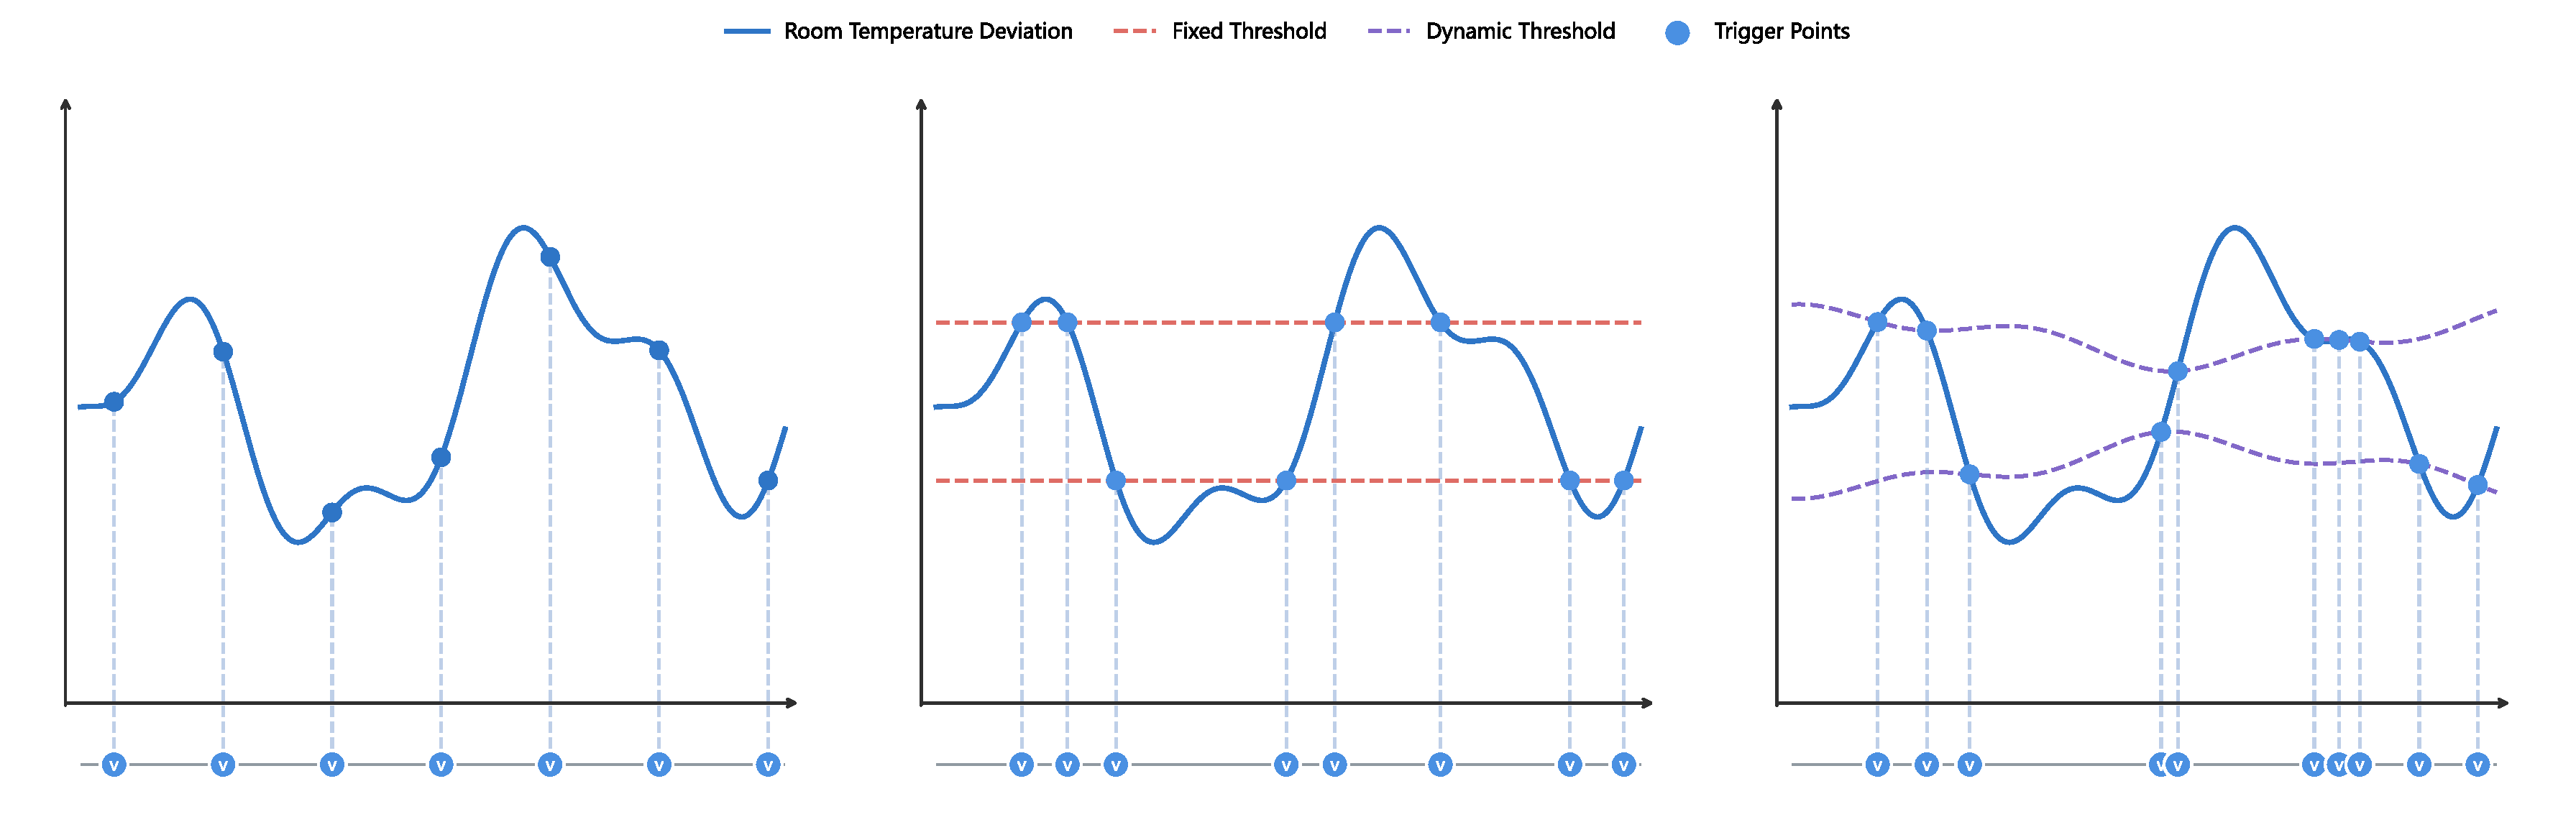
\includegraphics[width=\linewidth]{fig1_update_strategy_comparison.pdf}}
\caption{Comparison of fixed-interval, fixed-threshold, and dynamic-threshold update strategies. The top row shows the relationship between room temperature deviation signals and different trigger thresholds, and the bottom row shows the distribution of trigger times. Dashed markers indicate trigger times}\label{fig:update-strategy-comparison}
\end{figure}

Driven by the above motivations, we propose a new HVAC control method, event-triggered predictive reinforcement learning with unsupervised dynamic event gating (ET-PRL), that combines time-series prediction with unsupervised dynamic event gating in a deep reinforcement learning setting. ET-PRL learns event-triggering rules online from operational data through a data-driven method and activates a predictive reinforcement learning policy network to generate control actions when critical events are detected, allowing control sensitivity to adapt to different building characteristics and operating conditions. By integrating predictive features, adaptive gating, and the reinforcement learning controller within a unified method, ET-PRL preserves full control capability during major disturbances while reducing redundant updates during stable periods. The main contributions of this paper are as follows:

\begin{itemize}
\item
  We reformulate event triggering as an online anomaly detection problem, replacing manually defined static rules with an adaptive trigger criterion based on state deviation.
\item
  We develop unsupervised dynamic event gating by constructing a multi-scale fused anomaly score and a local-global two-layer adaptive threshold.
\item
  We establish a predictive RL control algorithm with dynamic event triggering, reducing redundant control updates while maintaining performance during stable periods.
\item
  We validate ET-PRL on real chiller operation data, demonstrating reduced action updates, improved energy efficiency, and a favorable balance between control performance and execution cost.
\end{itemize}

\section{Related Work}\label{related-work}

Coordinated control of energy efficiency and thermal comfort in building HVAC systems has long been a major engineering challenge. To address rising building energy demand and requirements for stable operation, early studies mainly relied on classic methods such as rule-based control (RBC) and proportional-integral-derivative (PID) control \cite{ref12}. Choi et al.~\cite{ref13} improved the practicality of HVAC rule-based control through optimization-informed rule extraction. Lee et al.~\cite{ref14} used deep reinforcement learning to tune PID parameters and improve tracking performance. Chojecki et al.~\cite{ref15} further introduced fuzzy control to improve adaptability under specific operating conditions. Tang et al.~\cite{ref16} proposed a physics-aware deep learning-embedded model predictive control (MPC) approach, which builds predictive models of building thermal dynamics and solves constrained optimization problems over a receding horizon to explicitly coordinate energy use, comfort, and equipment constraints. Although these methods are easy to deploy and reliable in industrial scenarios, or can achieve strong control performance when the model is accurate, they still depend on static rules, linear feedback assumptions, or high-fidelity predictive models. As a result, they have limited ability to represent nonlinear coupling, time-varying disturbances, and long thermal delays in buildings, and they often struggle to maintain both energy savings and comfort under complex operation and maintenance conditions \cite{ref17}.

To overcome the modeling and adaptability limits of traditional control, data-driven methods have become an important direction for intelligent HVAC control. Among them, reinforcement learning (RL) can learn optimized mappings between operating states and control actions through trial-and-error interaction with the building environment without requiring an accurate physical model, and has therefore been increasingly applied to building energy management, HVAC control, and demand response tasks \cite{ref18}. Savino et al.~\cite{ref19} demonstrated the potential of deep reinforcement learning for low-level control in multi-zone buildings. Wang et al.~\cite{ref20} and Zhuang et al.~\cite{ref21} used Deep Q-Network (DQN) and Deep Deterministic Policy Gradient (DDPG) based frameworks to learn mappings from high-dimensional sensor states to control actions, confirming the optimization benefits of reinforcement learning in complex scenarios. However, most reinforcement learning methods rely mainly on current observations, which can lead to control delay and oscillation in systems with strong thermal inertia and time lag \cite{ref22}. To mitigate this issue, Li et al.~\cite{ref23} integrated temporal models such as Long Short-Term Memory (LSTM) into the decision process, improving awareness of system evolution and partially improving control stability; He et al.~\cite{ref24} further developed a model-free predictive reinforcement learning (PRL) method for chiller plant optimization by combining LSTM-based load prediction with DQN control, showing that predictive information can improve control foresight while preserving the adaptability of RL. Nevertheless, existing RL and PRL methods still generally follow the TTC paradigm at the execution level, where states are sampled and actions are updated at preset intervals. This makes it difficult to adapt the decision frequency to the intensity of load disturbances and leads to an inherent conflict between redundant computation and actuator wear \cite{ref25}.

As control strategies have evolved from rule-driven to data-driven methods, reducing redundant computation and actuator wear has become another key issue. Liu et al.~\cite{ref26} showed that event-triggered control (ETC) updates control and communication only when the state exceeds a threshold or a defined event occurs, thereby reducing unnecessary updates in TTC. Fu et al.~\cite{ref9} further proposed ED-DQN, an event-driven deep reinforcement learning control method for multi-zone residential building HVAC systems, which introduces event triggering into DRL so that the agent updates control actions only when predefined events occur, thereby reducing redundant decisions under fixed-step control. Liu et al.~\cite{ref27} pointed out that ETC methods in practical deployment still rely heavily on expert-defined static threshold rules. Under non-stationary factors such as drift in building thermal characteristics, climate variation, and equipment aging, fixed thresholds usually cannot balance sensitivity and stability, which can lead to excessive triggering or delayed responses and thus weaken computational efficiency and comfort performance \cite{ref28}.

Building on these studies, we reformulate HVAC event triggering as an online unsupervised anomaly detection problem and propose event-triggered predictive reinforcement learning with unsupervised dynamic event gating (ET-PRL), an on-demand method that combines dynamic gating with predictive reinforcement learning. Compared with traditional static-rule methods and existing ETC schemes, ET-PRL introduces streaming feature tracking and adaptive thresholding to update triggering conditions dynamically, reducing dependence on manual tuning and improving adaptability to long-term drift. Unlike fixed-step reinforcement learning, the method further decouples decision timing through event-driven execution, thereby reducing redundant inference and equipment wear while using predictive features to compensate for the loss of state information caused by sparse control. As a result, ET-PRL achieves a practical balance between control performance and execution cost under non-stationary building operating conditions.

\section{Methodology}\label{methodology}

Given the thermal inertia and delayed response of building HVAC systems, together with distribution shift caused by seasonal changes in operating conditions, traditional event-triggered control methods that rely on offline calibration and static thresholds usually require frequent recalibration when transferred across scenarios, which increases engineering maintenance cost. To address this issue, we propose event-triggered predictive reinforcement learning with unsupervised dynamic event gating (ET-PRL), an on-demand control method that couples streaming anomaly gating with DRL. The overall architecture of the proposed method is shown in Figure~\ref{fig:et-prl-architecture}.

\begin{figure}
\centering
\pandocbounded{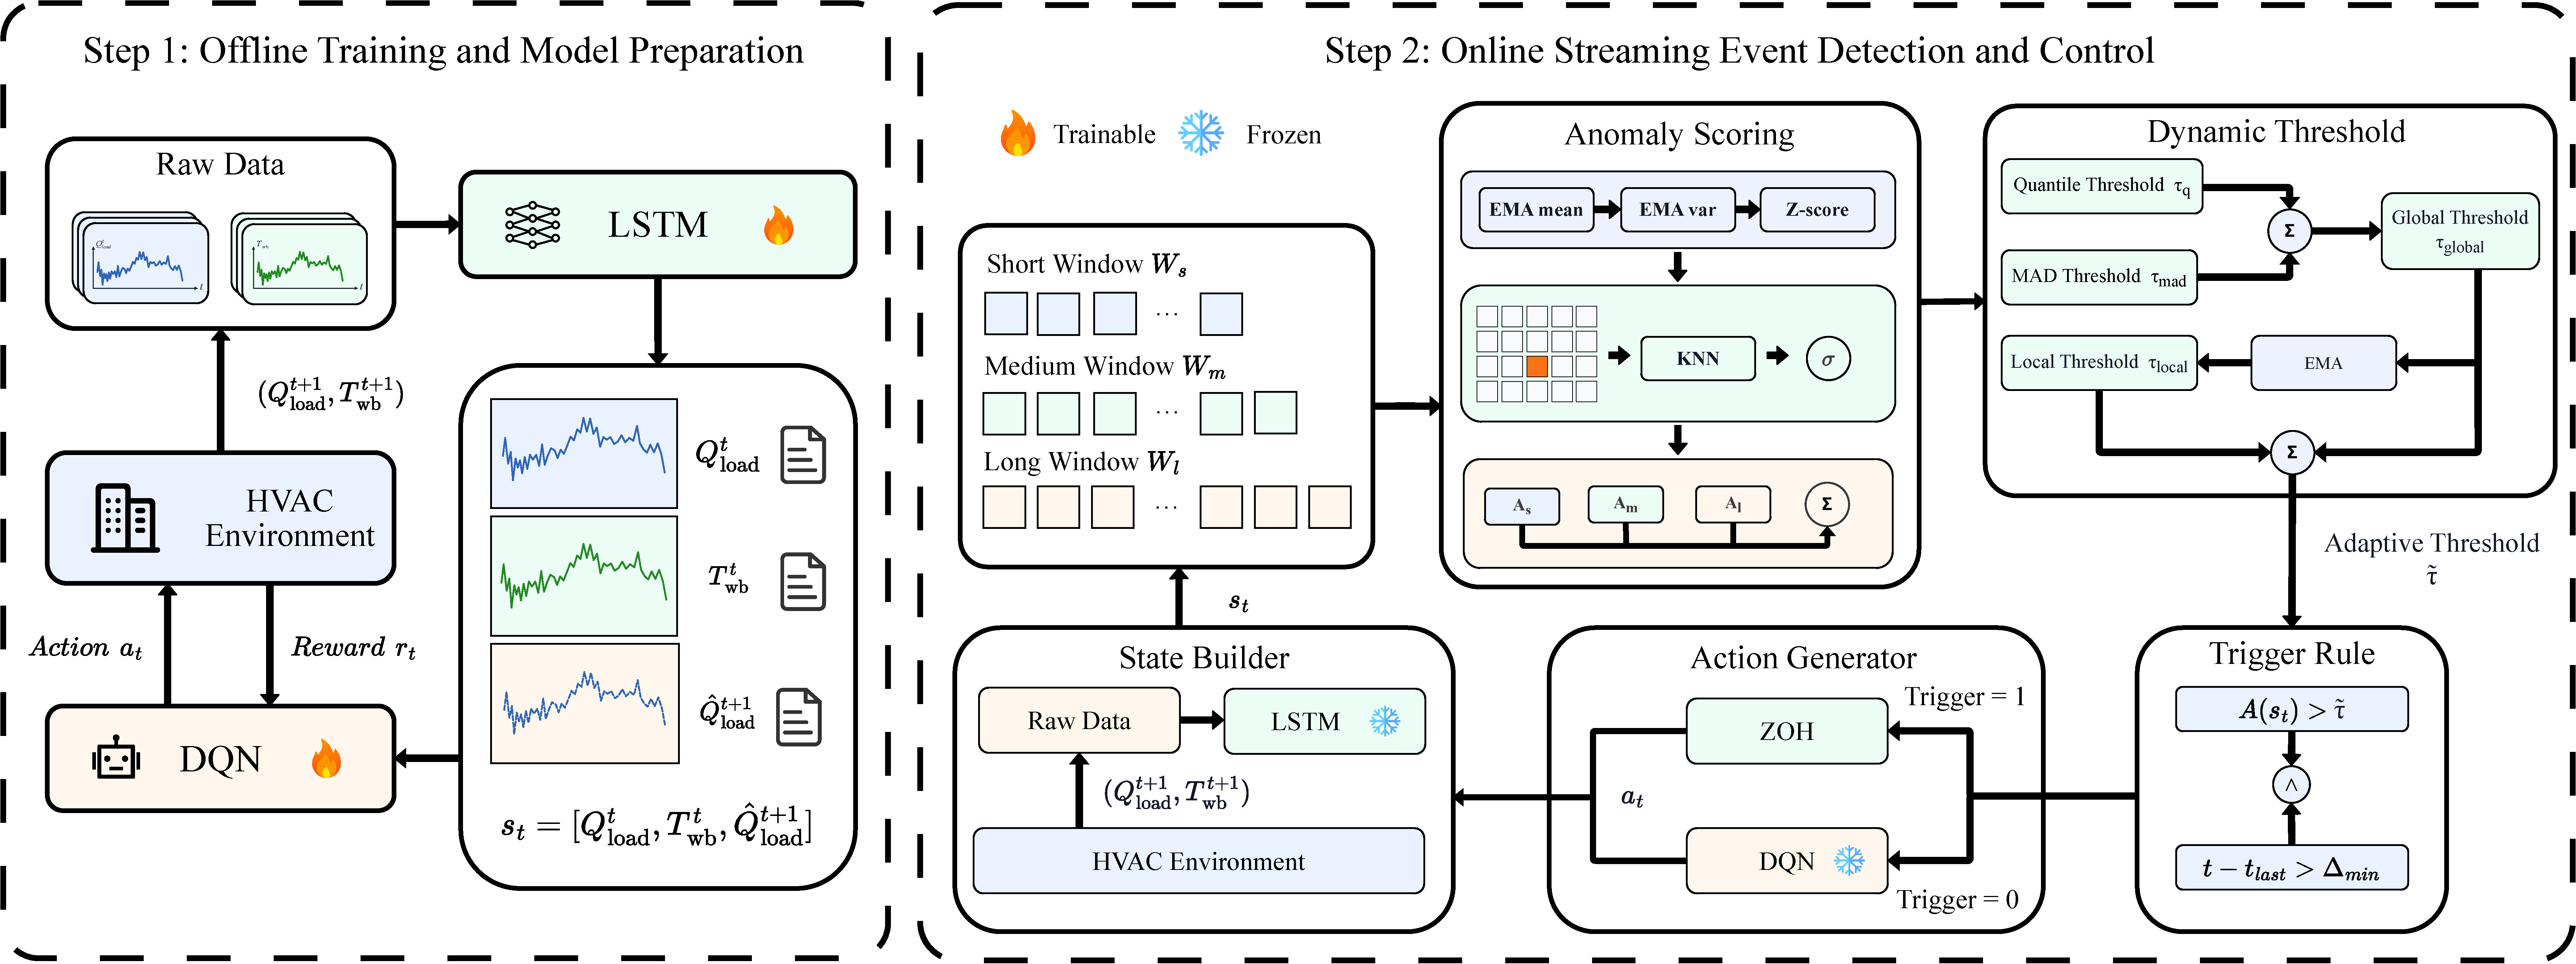
\includegraphics[width=\linewidth]{fig2_plain.pdf}}
\caption{Architecture of the proposed ET-PRL method, comprising offline training and model preparation (Step 1) and online streaming event detection and control (Step 2)}\label{fig:et-prl-architecture}
\end{figure}

In Step 1, historical operating data are used to train the load prediction model and the DQN policy offline. The LSTM provides a one-step-ahead cooling load estimate, which is combined with the current cooling load and outdoor wet-bulb temperature to form the compact state used by the controller. After training, both models are kept fixed during online deployment.

In Step 2, real-time measurements are continuously converted into the current state and passed to the online streaming gate. The gate compares the current operating condition with recent patterns through multi-scale tracking and an adaptive threshold, and then determines whether a new control update is needed. If an event is triggered, the DQN generates a new chilled water supply temperature setpoint. Otherwise, the previous setpoint is held by zero-order hold (ZOH). In this way, the method remains responsive during significant operating changes while reducing redundant updates during stable operation.

\subsection{Dynamic Event Triggering Design Based on Streaming Feature Tracking}\label{dynamic-event-triggering-design-based-on-streaming-feature-tracking}

In event-triggered control, activating a control update depends on identifying critical events, that is, moments when the system state deviates significantly from normal operation and demands prompt control action. Most existing methods define such events using manually preset static rules, which are difficult to adapt to nonlinear and time-varying characteristics of building HVAC systems. We reformulate critical event identification as an online anomaly detection problem. Specifically, in control terms, critical events correspond to abrupt operating condition shifts that require immediate control intervention, while in statistical terms, such moments usually appear as significant deviations of state samples from the normal distribution. Therefore, event judgment can be uniformly modeled as a deviation test rather than relying on manually defined static rules.

Let the system state feature vector be \(s_t\in\mathbb{R}^d\), the event label be \(e_t\in\{0,1\}\), and the normal reference distribution at time step \(t\) be denoted by \(\mathcal{P}^{\text{norm}}_t\). The event set is defined as Eq.~\eqref{eq:event-set}:

\[
\mathcal{E}_t=\{s:\,d(s,\mathcal{P}^{\text{norm}}_t)>\delta_t\},\qquad
e_t=\mathbb{I}(s_t\in\mathcal{E}_t) \tag{1}\label{eq:event-set}
\]

\noindent where \(\mathbb{I}(\cdot)\) is the indicator function that equals 1 when the condition holds and 0 otherwise; \(d(\cdot)\) denotes the distribution deviation metric, and \(\delta_t\) is the decision threshold. This definition shows that event detection is essentially a binary test of whether the current state deviates from the normal region. The control action is updated when the state enters a high-deviation region; otherwise, the current control action is maintained.

To convert distribution-level deviation testing into a scalar decision rule that can be updated in a streaming manner, an anomaly score function \(A(s_t)\) is used as a scalar proxy for the distribution deviation metric \(d(s,\mathcal{P}^{\text{norm}}_t)\), and the set-based rule is converted into a computable threshold comparison as Eq.~\eqref{eq:score-threshold-rule}: \[
e_t=\mathbb{I}(A(s_t)>\tau_t) \tag{2}\label{eq:score-threshold-rule}
\]

\noindent where a larger \(A(s_t)\) indicates a stronger deviation from normal behavior, and \(\tau_t\) is the trigger threshold, which is the computable counterpart of the decision threshold \(\delta_t\) in Eq.~\eqref{eq:event-set} expressed in the anomaly score space. This form has two advantages: First, it can be directly coupled with streaming statistics and updated step by step. Second, it is naturally consistent with the subsequent gating logic and enables integrated modeling and implementation from anomaly scoring to trigger decision.

Considering the non-stationarity caused by weather disturbances, equipment aging, and load behavior drift during long-term HVAC operation, the threshold is updated through a streaming adaptive mechanism rather than fixed value as Eq.~\eqref{eq:threshold-update}:

\[
    \tau_t=\Phi\big(A(s_{1}),\ldots,A(s_{t-1})\big) \tag{3}\label{eq:threshold-update}
\]

\noindent where \(\Phi(\cdot)\) denotes the threshold update operator driven by historical anomaly scores which balances sensitivity and stability. It increases event coverage when disturbances intensify and suppresses redundant triggering during steady periods, thereby reducing the risk of false triggers and missed triggers.

\paragraph{(1) Definition of System State Features}\label{definition-of-system-state-features}

The event gating module and the reinforcement learning controller share the same state feature which is defined as a compact three-dimensional feature vector as Eq.~\eqref{eq:state-vector-gate}:

\[s_t=[Q_{\mathrm{load}}^t,\,T_{\mathrm{wb}}^t,\,\hat{Q}_{\mathrm{load}}^{t+1}] \tag{4}\label{eq:state-vector-gate}\]

\noindent where, at time step \(t\), \(Q_{\mathrm{load}}^t\) denotes the system cooling load, \(T_{\mathrm{wb}}^t\) denotes the outdoor wet-bulb temperature, and \(\hat{Q}_{\mathrm{load}}^{t+1}\) denotes the one-step-ahead short-term prediction of the system cooling load.

The main reason for selecting \(T_{\mathrm{wb}}^t\) is that it can capture both ambient temperature and humidity and directly constrain cooling tower heat transfer performance and the upper limit of system heat rejection. It therefore serves as a key state variable for characterizing the intensity and direction of exogenous weather disturbances, which improves the ability of the gating mechanism to detect non-stationary environmental changes. Moreover, \(\hat{Q}_{\mathrm{load}}^{t+1}\) is selected because building thermal systems exhibit strong thermal inertia and control delay. If the gating mechanism relies only on current observations, trigger decisions usually lag behind operating condition shifts. By incorporating one-step-ahead load information, the gating module can sense rising or falling load trends earlier to some extent and trigger control action updates earlier during critical transitions, thereby reducing the risk of delayed response under sparse triggering.

\paragraph{(2) Streaming Isolation Depth and Multi-Scale Anomaly Tracking}\label{streaming-isolation-depth-and-multi-scale-anomaly-tracking}

Traditional offline anomaly detection usually depends on a static sample library and is less stable under seasonal operating drift. To address this issue, a streaming isolation depth mechanism is deployed to score anomalies of the online system state feature \(s_t\) in real time. Streaming Isolation Depth dynamically builds and updates isolation tree structures over sliding data windows, and uses the average path length of a sample across multiple trees to measure its degree of isolation. A shorter path means the sample is easier to isolate and therefore more likely to be anomalous. This mechanism can adapt to distribution changes online without retraining a global model.

Each isolation tree isolates data points by recursively selecting random features and split state points. For a state point \(s_t\), search is performed on \(\psi\) isolation trees built from the sliding reference window, and \(h_j(s_t)\) denotes the path length on the \(j\)-th tree, where the path length is defined as the number of edges from the root node to the leaf node. The average isolation depth of the sample is defined as Eq.~\eqref{eq:isolation-depth}:

\[h_{\mathrm{iso}}(s_t) = \frac{1}{\psi} \sum_{j=1}^{\psi} h_j(s_t) \tag{5}\label{eq:isolation-depth}\]

Thereafter, \(h_{\mathrm{iso}}(s_t)\) is further converted into a normalized anomaly score as Eq.~\eqref{eq:isolation-score}, where \(m\) is the number of samples in the reference set and \(C(m)\) is the corresponding baseline for average path length.

\[A_{\mathrm{iso}}(s_t) = 2^{-\frac{h_{\mathrm{iso}}(s_t)}{C(m)}} \tag{6}\label{eq:isolation-score}\]

The normalization constant is computed as \(C(m) = 2H(m-1) - \frac{2(m-1)}{m}\), where \(H(m-1)=\sum\limits_{i=1}^{m-1}\frac{1}{i}\) is the harmonic series which maps the anomaly score to the interval \((0,1)\): shorter paths yield scores closer to 1, indicating easy isolation, whereas longer paths yield scores closer to 0, indicating difficulty of isolation.

The computation process maintains three sliding reference windows of different sizes to form multi-scale dynamic reference sets. The short window \(\mathcal{W}_{\mathrm{short}}\) contains the most recent \(n_s\) data points and is used to capture high-frequency fluctuations. The medium window \(\mathcal{W}_{\mathrm{medium}}\) contains the most recent \(n_m\) data points and is used to represent the intraday cycle. The long window \(\mathcal{W}_{\mathrm{long}}\) contains the most recent \(n_l\) data points and is used to describe seasonal drift, with \(n_s < n_m < n_l\). Isolation trees are applied independently to each window, and an anomaly score is produced at each scale at every time step. Let \(\kappa\in\{\mathrm{short},\mathrm{medium},\mathrm{long}\}\) and let \(n_\kappa\) denote the corresponding window size. The corresponding scale-specific anomaly score is given by Eq.~\eqref{eq:scale-specific-score}:

\[A_{\kappa}(s_t)=2^{-\frac{h_{\mathrm{iso}}^{\kappa}(s_t)}{C(n_{\kappa})}} \tag{7}\label{eq:scale-specific-score}\]

All scale-specific scores are normalized to the interval \([0,1]\). The overall anomaly score is defined as a weighted fusion of the three scale-specific scores as Eq.~\eqref{eq:multi-scale-score}.

\[A(s_t)=w_{\mathrm{s}}A_{\mathrm{short}}(s_t)+w_{\mathrm{m}}A_{\mathrm{medium}}(s_t)+w_{\mathrm{l}}A_{\mathrm{long}}(s_t) \tag{8}\label{eq:multi-scale-score}\]

\noindent where \(w_{\mathrm{s}}, w_{\mathrm{m}}, w_{\mathrm{l}} \ge 0\) and \(w_{\mathrm{s}}+w_{\mathrm{m}}+w_{\mathrm{l}}=1\), which represent the fusion weights of the corresponding timescales.

We construct the composite anomaly score through weighted fusion of short, medium, and long timescales. The short-term scale primarily captures high-frequency disturbances, the medium-term scale characterizes intraday periodic variations, and the long-term scale tracks seasonal drift and long-term slow processes. This multi-scale fusion mechanism enables the gating module to jointly respond to local abrupt disturbances and system-level slow-varying trends, avoiding the insufficient sensitivity or excessive triggering that a single-scale statistic may exhibit under non-stationary operating conditions, thereby improving the adaptability and robustness of the gating mechanism across diverse operating scenarios.

\paragraph{(3) Streaming Two-Layer Adaptive Threshold Optimization}\label{streaming-two-layer-adaptive-threshold-optimization}

Eq.~\eqref{eq:multi-scale-score} provides the multi-scale fused anomaly score \(A(s_t)\), but the triggering decision still requires comparing this score against a threshold \(\tau_t\), as defined in Eq.~\eqref{eq:score-threshold-rule}. Under long-term non-stationary HVAC operation, a fixed threshold is prone to either insufficient sensitivity or excessive triggering, whereas a single adaptive statistic cannot simultaneously accommodate rapid response to short-term disturbances and stable tracking of long-term drift. To resolve this issue, we construct a local-global two-layer adaptive threshold that achieves adaptive triggering through coordinated fast- and slow-timescale updates.

Specifically, we first estimate the upper-tail boundaries of the empirical anomaly score distribution within the sliding window using the upper quantile and the median absolute deviation (MAD) respectively, and then fuse them into a candidate threshold via weighted combination. A local exponential smoothing step is subsequently applied to this candidate threshold, yielding a local threshold that tracks recent operating condition changes. To capture longer-term trends, we further introduce a global threshold with a slower update rate, which serves as a smooth baseline constraint against drift. The final triggering threshold is determined by combining both the local and global components rather than relying on a single statistic, which enables the gating mechanism to jointly maintain short-term responsiveness and long-term stability across non-stationary operating conditions.

To reduce the influence of anomalous samples on location and scale statistics, we employ two robust statistics to construct the candidate threshold: an upper-quantile-based threshold \(\tau_q^{(t)}\) and a median absolute deviation (MAD)-based threshold \(\tau_{\mathrm{mad}}^{(t)}\). The former captures the upper-tail position of the empirical anomaly score distribution, while the latter characterizes the robust dispersion around the median defined as Eqs.~\eqref{eq:quantile-threshold} and \eqref{eq:mad-threshold}:

\[\tau_{q}^{(t)}=Q_q(\mathcal{A}_t^{(W)}) \tag{9}\label{eq:quantile-threshold}\]

\[\begin{aligned}
\tau_{\mathrm{mad}}^{(t)} &= \operatorname{med}(\mathcal{A}_t^{(W)})+\kappa \cdot c \cdot \operatorname{MAD}(\mathcal{A}_t^{(W)}) \\
&= \operatorname{med}(\mathcal{A}_t^{(W)})+\kappa \cdot c \cdot\operatorname{med}\left(\left\{\left|a-\operatorname{med}(\mathcal{A}_t^{(W)})\right|:a\in\mathcal{A}_{t}^{(W)}\right\}\right)
\end{aligned} \tag{10}\label{eq:mad-threshold}\]

\noindent where \(\mathcal{A}_t^{(W)}=\{A(s_{t-W+1}),\ldots,A(s_t)\}\) denotes the anomaly score sliding window of length \(W\); \(Q_q(\cdot)\) is the empirical quantile at level \(q\in(0.5,1)\); \(\operatorname{med}(\cdot)\) is the median function; \(\kappa\) is the sensitivity coefficient; and \(c \approx 1.4826\) is the consistency constant for Gaussian distributions. The threshold \(\tau_q^{(t)}\) primarily characterizes the upper-tail position of the empirical anomaly score distribution, whereas \(\tau_{\mathrm{mad}}^{(t)}\) refines this boundary according to the robust dispersion of scores within the window.

On this basis, we construct the local candidate threshold to provide an initial estimate of the triggering boundary for the historical window defined as Eq.~\eqref{eq:candidate-threshold}:

\[\tau_{\mathrm{cand}}^{(t)}=\omega_q\tau_q^{(t)}+(1-\omega_q)\tau_{\mathrm{mad}}^{(t)} \tag{11}\label{eq:candidate-threshold}\]

\noindent where \(\omega_q \in [0,1]\) is the fusion weight. A larger \(\omega_q\) shifts the candidate threshold closer to the upper-quantile boundary, making the criterion more dependent on whether the current anomaly score exceeds the high-quantile level within the historical window. A smaller \(\omega_q\) takes greater emphasis on the robust fluctuation scale reflected by MAD, thereby increasing sensitivity to expansion or contraction of the score distribution.

As \(\tau_{\mathrm{cand}}^{(t)}\) may still be affected by single-step spike disturbances, we further apply exponential smoothing on a fast timescale to obtain the local threshold as Eq.~\eqref{eq:local-threshold}:

\[\tau_{\mathrm{local}}^{(t)}=(1-\lambda_{\mathrm{local}})\tau_{\mathrm{local}}^{(t-1)}+\lambda_{\mathrm{local}}\tau_{\mathrm{cand}}^{(t)} \tag{12}\label{eq:local-threshold}\]

\noindent where \(\lambda_{\mathrm{local}} \in (0,1]\) is the local update rate, and \(\tau_{\mathrm{local}}^{(0)}=\tau_{\mathrm{cand}}^{(t_0)}\) with \(t_0\) denoting the first time step at which a complete sliding window is available. By applying first-order smoothing, \(\tau_{\mathrm{local}}^{(t)}\) achieves a trade-off between threshold responsiveness and resistance to jitter. A larger \(\lambda_{\mathrm{local}}\) enables the local threshold to follow recent operating condition transitions more rapidly, whereas a smaller \(\lambda_{\mathrm{local}}\) makes the local threshold less sensitive to short-duration impulsive noise.

When the system undergoes slow drift due to seasonal variation, equipment aging, or shifts in operating boundaries, the local threshold may be gradually pulled by long-term changes, thereby weakening its ability to detect sustained distributional shifts. We therefore construct a global threshold on a slower timescale as a long-term baseline reference as Eq.~\eqref{eq:global-threshold}:

\[\tau_{\mathrm{global}}^{(t)}=(1-\lambda_{\mathrm{global}})\tau_{\mathrm{global}}^{(t-1)}+\lambda_{\mathrm{global}}\tau_{\mathrm{local}}^{(t)} \tag{13}\label{eq:global-threshold}\]

\noindent where \(\tau_{\mathrm{global}}^{(0)}=\tau_{\mathrm{local}}^{(0)}=\tau_{\mathrm{cand}}^{(t_0)}\) and \(\lambda_{\mathrm{global}} \ll \lambda_{\mathrm{local}}\), ensuring that the global threshold exhibits stronger smoothness and hysteresis.

The final streaming two-layer adaptive threshold is obtained by fusing the local and global thresholds as Eq.~\eqref{eq:streaming-threshold}:

\[\tilde{\tau}_t=\alpha_{\mathrm{local}}\tau_{\mathrm{local}}^{(t)}+(1-\alpha_{\mathrm{local}})\tau_{\mathrm{global}}^{(t)}+b_{\mathrm{bias}} \tag{14}\label{eq:streaming-threshold}\]

\noindent where \(\alpha_{\mathrm{local}}\in[0,1]\) controls the blending ratio between short-term and long-term information. Increasing \(\alpha_{\mathrm{local}}\) shifts the final threshold toward recent operating conditions, yielding more responsive triggering behavior; decreasing it shifts the threshold toward the long-term baseline, yielding more stable judgment. The term \(b_{\mathrm{bias}}\in[-1, 1]\) is a global offset correction that compensates for potential systematic bias arising from finite-window estimation at different operating stages. During highly stable phases such as nighttime low-load periods, the triggering boundary computed solely from local and global statistics may be biased due to window effects, leading to frequent boundary oscillations. Incorporating this offset therefore improves the robustness of the decision criterion.

\subsection{Online Streaming Event Gating Module Construction}\label{online-streaming-event-gating-module-construction}

After obtaining the basic adaptive gating threshold \(\tilde{\tau}_t\), we further convert it into an actionable triggering criterion. Unlike traditional fixed-threshold or single-condition exceedance triggering strategies, our gating module employs a joint determination form that combines anomaly intensity discrimination with time-constraint oscillation suppression. The objective is to guarantee coverage of critical disturbances while suppressing chatter triggering near threshold boundaries. The former component evaluates the current state deviation by comparing \(A(s_t)\) against the adaptive threshold, whereas the latter explicitly regulates the action update frequency through a minimum trigger interval constraint. This design prevents consecutive triggering caused by short-term high-frequency fluctuations, which would otherwise lead to frequent setpoint switching and actuator wear.

At each control time step, the gating module receives the current system state feature \(s_t\), computes the anomaly score \(A(s_t)\), and performs a binary trigger determination as Eqs.~\eqref{eq:trigger-threshold} and \eqref{eq:trigger-rule}:

\[\tau_t^*=\operatorname{clip}(\tilde{\tau}_t+m_{\mathrm{hys}},0,1) \tag{15}\label{eq:trigger-threshold}\]

\[\mathrm{Trigger}(s_t)=\mathbb{I}\left(A(s_t)>\tau_t^*\right)\land\mathbb{I}\left(t-t_{\mathrm{last}}>\Delta_{\min}\right) \tag{16}\label{eq:trigger-rule}\]

\noindent where \(\tilde{\tau}_t\) is the streaming two-layer adaptive threshold defined in Eq.~\eqref{eq:streaming-threshold}, \(\operatorname{clip}(\cdot, 0, 1)\) constrains the input value to the interval \([0,1]\), \(m_{\mathrm{hys}}\) is a hysteresis margin that prevents the trigger signal from repeatedly flipping near the threshold boundary, \(t_{\mathrm{last}}\) records the time step at which the system last triggered a control action update, and \(\Delta_{\min}\) is the specified minimum trigger interval. When \(\mathrm{Trigger}(s_t)=1\), the gating module triggers PRL module to generate a new control action for the current time step, and when \(\mathrm{Trigger}(s_t)=0\), the control action from the previous time step is held via a zero-order hold.

Regardless of the value of \(\mathrm{Trigger}(s_t)\), the gating module executes anomaly score window maintenance and two-layer threshold recursive update at every time step. Specifically, after performing the trigger determination in Eq.~\eqref{eq:trigger-threshold}, we append the current anomaly score \(A(s_t)\) to the sliding window \(\mathcal{A}_t^{(W)}\) and sequentially update the candidate threshold, local threshold, and global threshold according to Eqs.~\eqref{eq:candidate-threshold}--\eqref{eq:streaming-threshold}, thereby providing the most recent statistical reference baseline for the next time step. Through the update, the gating module's threshold estimation is always grounded in the latest observations, thereby preventing the statistics from lagging behind operating condition changes due to trigger sparsification and guaranteeing that the trigger sensitivity can be promptly restored once a stable period ends and disturbances intensify.

\subsection{Predictive RL Control Algorithm with Dynamic Event Triggering}\label{predictive-rl-control-algorithm-with-dynamic-event-triggering}

Based on the trigger signal provided by the gating module, we construct a lightweight DQN agent augmented with short-term load prediction as the RL controller, balancing control performance against online computational cost. Once the trigger happens, the controller receives the state vector \(s_t\) and a composite reward \(r_t\), outputs a chilled water supply temperature setpoint that trades off energy reduction with temperature tracking quality. Moreover, we adopt a hierarchical execution strategy that decouples the high-level model-free optimization decisions from the low-level physical operating constraints of the equipment, ensuring that the generated actions satisfy engineering requirements such as unit start/stop sequencing and minimum run-time durations.

\paragraph{(1) Task formulation and problem definition}\label{task-formulation-and-problem-definition}

To address high-dimensional state spaces and strong temporal correlations among samples in HVAC control, we adopt a compact state representation and formulate the control problem as an MDP \(\langle \mathcal{S}, \mathcal{A}, \mathcal{P}, \mathcal{R}, \gamma \rangle\), where \(\mathcal{S}\) denotes the state space, \(\mathcal{A}\) denotes the action space, \(\mathcal{P}\) denotes the state transition kernel, \(\mathcal{R}\) denotes the reward function, and \(\gamma\) denotes the discount factor.

The state vector \(s_t \in \mathcal{S}\) is defined by Eq.~\eqref{eq:mdp-state}:

\[s_t = [Q_{\mathrm{load}}^t, T_{\mathrm{wb}}^t, \hat{Q}_{\mathrm{load}}^{t+1}] \tag{17}\label{eq:mdp-state}\]

\noindent where \(Q_{\mathrm{load}}^t\) denotes the system cooling load at time step \(t\), \(T_{\mathrm{wb}}^t\) denotes the outdoor wet-bulb temperature at time step \(t\), and \(\hat{Q}_{\mathrm{load}}^{t+1}\) denotes the short-term prediction of the system cooling load at the next time step. The MDP state vector \(s_t\) uses the same feature components as the input state feature vector of the gating module in Eq.~\eqref{eq:state-vector-gate}. By incorporating \(\hat{Q}_{\mathrm{load}}^{t+1}\), we add forward-looking load information to the compact state representation, which helps characterize short-term load trends and improves the representation of load dynamics without substantially increasing the state dimension. Longer timescale dynamics that are not explicitly included in the state vector are further characterized by the multi-scale statistics maintained within the gating mechanism.

We define the action \(a_t\) as the chilled water supply temperature setpoint at time step \(t\) which takes one of 10 discrete values within \([6,15]^{\circ}\mathrm{C}\) and directly determines the operating target of the cooling system. Consistent with the compact state representation, we formulate the control decision as a single setpoint to avoid the training complexity and online inference cost associated with a high-dimensional action space. The upper-level RL module generates action adaptively according to the current state, while the lower-level rule-based module coordinates and constrains engineering requirements that are not directly decided by the agent, such as unit startup and shutdown sequencing and minimum runtime constraints.

We define the reward \(r_t\) by Eq.~\eqref{eq:reward} as a weighted sum of an energy efficiency term and a temperature tracking term, so that the learned policy can balance energy saving with setpoint tracking:

\[r_t = \omega_{\eta} r_t^{\mathrm{energy}} + \omega_{\tau} r_t^{\mathrm{track}} \tag{18}\label{eq:reward}\]

\noindent where \(\omega_{\eta},\omega_{\tau}\ge 0\) and \(\omega_{\eta}+\omega_{\tau}=1\) denote the weights assigned to the energy efficiency and temperature tracking terms, respectively. A larger \(\omega_{\eta}\) guides the policy toward energy saving, whereas a larger \(\omega_{\tau}\) gives greater priority to temperature tracking. The energy efficiency term is calculated by Eq.~\eqref{eq:energy-reward}:

\[r_t^{\mathrm{energy}} = 1 - \frac{P_t}{P_{\mathrm{ref}}} \tag{19}\label{eq:energy-reward}\]

\noindent where \(P_t\) is the instantaneous operating power of the chiller unit and \(P_{\mathrm{ref}}\) is the rated power. This term evaluates the current power demand relative to the rated power. A lower operating power therefore produces a higher reward. We calculate the temperature tracking term using the Gaussian radial basis function in Eq.~\eqref{eq:tracking-reward}, which provides a continuous measure of setpoint tracking accuracy:

\[r_t^{\mathrm{track}} = \exp \left( -\frac{1}{2} \left( \frac{T_t - T_{\mathrm{set}}}{\sigma} \right)^2 \right) \tag{20}\label{eq:tracking-reward}\]

\noindent where \(T_t\) is the actual supply water temperature, \(T_{\mathrm{set}}\) is the target setpoint temperature, and \(\sigma\) is the Gaussian kernel bandwidth parameter, which controls the sensitivity of the reward to temperature deviations. This term takes a larger value when the actual supply temperature is closer to the target setpoint, thereby encouraging the control policy to maintain stable temperature regulation.

\paragraph{(2) Predictive DQN network architecture and training procedure}\label{predictive-dqn-network-architecture-and-training-procedure}

We formulate the chilled water supply temperature setpoint optimization process as an action-value function approximation problem over a discrete action space and employ a predictive DQN controller to solve it. A multi-layer fully connected network approximates the action-value function \(Q_{\theta}\), where \(\theta\) denotes the parameters of the online network. The network takes the state vector \(s_t\) defined by Eq.~\eqref{eq:mdp-state} as input and outputs the action value \(Q_{\theta}[s_t,a]\) for each candidate action \(a\) in the discrete action space \(\mathcal{A}\). Unlike reactive action selection that relies solely on current observations, the one-step load prediction term in the state enables \(Q_{\theta}\) to evaluate the long-term return of each candidate setpoint under the joint constraints of the current operating condition and short-term load evolution which can provide forward-looking action inference when an event is triggered.

We conduct offline training using chronologically ordered data splits to prevent leakage of future operating information and to match the sequential observation conditions encountered during deployment. The simulation environment maps state-action pairs to physical feedback through the chiller performance curves, cooling load, and outdoor wet-bulb temperature, and it computes the immediate reward \(r_t\) defined by Eqs.~\eqref{eq:reward}--\eqref{eq:tracking-reward}. Consequently, the parameter updates are jointly constrained by energy efficiency and temperature tracking performance. During training, we adopt an \(\epsilon\)-greedy action selection mechanism with a gradually decaying exploration rate to balance exploration of chilled water supply temperature setpoints against exploitation of learned action values.

We store each interaction sample \((s_t,a_t,r_t,s_{t+1})\) in an experience replay buffer \(\mathcal{D}\) with capacity \(M\), where \(a_t\) denotes the encoded discrete setpoint action. Once the number of stored samples reaches the batch size \(B\), we randomly draw mini-batches from \(\mathcal{D}\) for parameter updates, thereby reducing the temporal correlation among adjacent load samples. Consistent with the sequential replay implementation adopted in this work, we do not explicitly include a terminal mask in the target Q value \(y_t^{Q}\). Instead, we construct it from the immediate reward \(r_t\), the discount factor \(\gamma\), and the maximum action value of the next state under the target network parameters \(\theta^{-}\), where \(a'\) denotes a candidate discrete setpoint action at the next state \(s_{t+1}\). We define the target Q value \(y_t^{Q}\) by Eq.~\eqref{eq:target-q}:

\[y_t^{Q} = r_t + \gamma \max_{a' \in \mathcal{A}} Q_{\theta^{-}}[s_{t+1},a'] \tag{21}\label{eq:target-q}\]

We adopt the Smooth L1 loss for the training loss \(\mathcal{L}_{\theta}\) to mitigate the distorting effect of abrupt load changes and local nonlinearities in the chiller power model on gradient updates. Let \(\delta_t=Q_{\theta}[s_t,a_t]-y_t^{Q}\) denote the action-value estimation error, and let \(\ell_{\mathrm{SL1}}(\cdot)\) denote the Smooth L1 loss function. We specify the optimization objective for the online network parameters \(\theta\) by Eq.~\eqref{eq:smooth-l1-loss}:

\[\mathcal{L}_{\theta} = \mathbb{E}_{\mathcal{D}}\left[\ell_{\mathrm{SL1}}(\delta_t)\right] \tag{22}\label{eq:smooth-l1-loss}\]

We update the online network using the Adam optimizer and synchronize the target network with the online network at a fixed frequency. During training, we disable exploration on the validation sequence and evaluate the current policy by greedy action selection in terms of cumulative reward. If the validation reward shows no continuous improvement in the second half of training, we apply early stopping and retain the policy network with the best validation performance. The final DQN policy serves only for action inference during online operation: it outputs the chilled water supply temperature setpoint from the predictive state when an event is triggered.

\paragraph{(3) Event-driven online execution algorithm}\label{event-driven-online-execution-algorithm}

During online operation, the system directly collects the cooling load \(Q_{\mathrm{load}}^t\), outdoor wet-bulb temperature \(T_{\mathrm{wb}}^t\), and one-step-ahead predicted load \(\hat{Q}_{\mathrm{load}}^{t+1}\) from the building operating environment at a fixed sampling interval to construct the predictive state \(s_t\). The streaming gate then evaluates whether the current operating state deviates from the recent reference distribution represented by the multi-scale sliding windows. A new chilled water supply temperature setpoint is inferred from the trained DQN only when the triggering criterion is satisfied. By coupling multi-scale anomaly scoring with predictive reinforcement learning control, this design enables the controller to respond to load changes, outdoor thermal disturbances, and operating-condition transitions while reducing unnecessary policy evaluations, frequent setpoint switching, and actuator oscillation under stable conditions.

Specifically, the streaming gate first computes scale-specific anomaly scores over short-term, medium-term, and long-term sliding windows to characterize high-frequency disturbances, intraday periodic variations, and long-term slow drift. The scale-specific anomaly scores are fused according to Eq.~\eqref{eq:multi-scale-score} to obtain the multi-scale fused anomaly score \(A(s_t)\), and the local-global two-layer adaptive threshold defined by Eqs.~\eqref{eq:quantile-threshold}--\eqref{eq:trigger-rule} is used to obtain the adaptive triggering threshold \(\tau_t^*\). The trigger decision compares \(A(s_t)\) with \(\tau_t^*\) and further incorporates the minimum triggering interval \(\Delta_{\min}\) and the hysteresis margin to suppress repeated triggers caused by threshold-level fluctuations. If \(\mathrm{Trigger}(s_t)=1\), the current operating state is considered sufficiently different from the recent reference distribution to trigger new policy inference, and the trained DQN policy network selects the setpoint with the highest learned action value from the discrete action space \(\mathcal{A}\). If \(\mathrm{Trigger}(s_t)=0\), no new policy inference is performed, and the control action is held by a zero-order hold (ZOH), i.e., \(a_t = a_{t-1}\). Here, \(\pi_{\mathrm{DQN}}(s_t)=\arg\max_{a\in\mathcal{A}}Q_{\theta}(s_t,a)\) denotes the greedy action selected by the trained DQN given state \(s_t\). The online execution is defined by Eq.~\eqref{eq:online-action}:

\[a_t = \begin{cases}\pi_{\mathrm{DQN}}(s_t), & \mathrm{Trigger}(s_t) = 1 \\a_{t-1}, & \mathrm{Trigger}(s_t) = 0\end{cases} \tag{23}\label{eq:online-action}\]

The complete online execution procedure of the proposed ET-PRL method is summarized in the following pseudocode.

\begin{paperalgorithm}{ET-PRL online control procedure}
\algline{\textbf{Input:} Trained DQN policy $\pi_{\mathrm{DQN}}$; gate parameters $\Omega$; minimum trigger interval $\Delta_{\min}$; total control horizon $T$.}
\algline{Here, $\Omega=\{w_{\mathrm{s}},w_{\mathrm{m}},w_{\mathrm{l}},q,\kappa,\omega_q,\lambda_{\mathrm{local}},\lambda_{\mathrm{global}},\alpha_{\mathrm{local}},b_{\mathrm{bias}},W,m_{\mathrm{hys}}\}$ is defined in Eqs.~\eqref{eq:scale-specific-score}--\eqref{eq:trigger-rule}.}
\algline{\textbf{Output:} Control setpoint sequence $\{a_t\}_{t=1}^{T}$.}
\algline{\textbf{Initialization:}}
\algline[\paperalgindent]{Set the initial control action $a_0$.}
\algline[\paperalgindent]{Set the last trigger time $t_{\mathrm{last}}=-\infty$.}
\algline[\paperalgindent]{Initialize the anomaly score sliding window $\mathcal{A}_t^{(W)}$.}
\algline{\textbf{for} $t=1,\ldots,T$ \textbf{do}}
\algline[\paperalgindent]{Collect $Q_{\mathrm{load}}^t$, $T_{\mathrm{wb}}^t$, and $\hat{Q}_{\mathrm{load}}^{t+1}$.}
\algline[\paperalgindent]{Construct the predictive state $s_t=[Q_{\mathrm{load}}^t,T_{\mathrm{wb}}^t,\hat{Q}_{\mathrm{load}}^{t+1}]$.}
\algline[\paperalgindent]{Compute $A_{\mathrm{short}}(s_t)$, $A_{\mathrm{medium}}(s_t)$, and $A_{\mathrm{long}}(s_t)$.}
\algline[\paperalgindent]{Compute $A(s_t)$ according to Eq.~\eqref{eq:multi-scale-score}.}
\algline[\paperalgindent]{Compute the candidate, local, and global thresholds according to Eqs.~\eqref{eq:candidate-threshold}--\eqref{eq:streaming-threshold}.}
\algline[\paperalgindent]{Compute $\tau_t^*$ according to Eq.~\eqref{eq:trigger-threshold}.}
\algline[\paperalgindent]{\textbf{if} $A(s_t)>\tau_t^*$ and $t-t_{\mathrm{last}}>\Delta_{\min}$ \textbf{then}}
\algline[\paperalgsubindent]{Infer a new control setpoint using the trained DQN policy: $a_t=\pi_{\mathrm{DQN}}(s_t)$.}
\algline[\paperalgsubindent]{Update the last trigger time: $t_{\mathrm{last}}=t$.}
\algline[\paperalgindent]{\textbf{else}}
\algline[\paperalgsubindent]{Hold the previous control setpoint: $a_t=a_{t-1}$.}
\algline[\paperalgindent]{\textbf{end if}}
\algline[\paperalgindent]{Execute $a_t$.}
\algline[\paperalgindent]{Append $A(s_t)$ to $\mathcal{A}_t^{(W)}$ for the next threshold update.}
\algline{\textbf{end for}}
\end{paperalgorithm}

\section{Case System and Simulation Environment}\label{case-system-and-simulation-environment}

\subsection{Building Thermal System Modeling}\label{building-thermal-system-modeling}

We constructed an EnergyPlus model using data from a commercial building HVAC system in Shanghai as the simulation test platform. The model was calibrated in previous work using measured operational data and can reproduce the main thermodynamic response of the chilled water system \cite{ref29}. The cooling source system is a primary pump constant-flow chilled water system, mainly consisting of centrifugal chillers, chilled water pumps, cooling water pumps, and cooling towers. To ensure consistency between component parameters and the simulation model inputs, the rated parameters of the main equipment were configured according to the design specifications and the calibrated model parameters. The key design parameters of the system are listed in Table A.1 in Appendix A, where the coefficient of performance, COP, is defined as the ratio of cooling capacity to input power.

\subsection{Weather and Load Dataset Characteristics}\label{weather-and-load-dataset-characteristics}

We use a cooling load sequence directly collected from the operating environment of a commercial building HVAC system in Shanghai as \(Q_{\mathrm{load}}\), with a sampling interval of \(5\,\mathrm{min}\), and pair it with the outdoor wet-bulb temperature \(T_{\mathrm{wb}}\) on the same time axis to form the main state data. The period extends from July 1 to October 10, corresponding to \(102\) days, or \(29,376\) time steps at the \(5\,\mathrm{min}\) resolution, thereby capturing both intraday periodic fluctuations and seasonal-scale variations. Descriptive statistics show that the peak cooling load is \(5102.77\,\mathrm{kW}\), with a standard deviation of \(962.02\,\mathrm{kW}\) and a coefficient of variation (CV) of \(37.3\%\), while the outdoor wet-bulb temperature \(T_{\mathrm{wb}}\) ranges from \(21\) to \(28\,\mathrm{^{\circ}C}\).

Figure~\ref{fig:dataset-temporal-characteristics} presents the multi-scale temporal characteristics of the cooling load and outdoor wet-bulb temperature. In the representative 14-day segment shown in Figure~\ref{fig:dataset-temporal-characteristics}a, \(Q_{\mathrm{load}}\) and \(T_{\mathrm{wb}}\) generally increase and decrease together during high-load periods, although \(Q_{\mathrm{load}}\) exhibits a much larger diurnal amplitude. The time-of-day averaged profiles in Figure~\ref{fig:dataset-temporal-characteristics}b further show that \(Q_{\mathrm{load}}\) rises during daytime operating hours and decreases at night, whereas \(T_{\mathrm{wb}}\) varies more smoothly over the day.

\begin{figure}
\centering
\pandocbounded{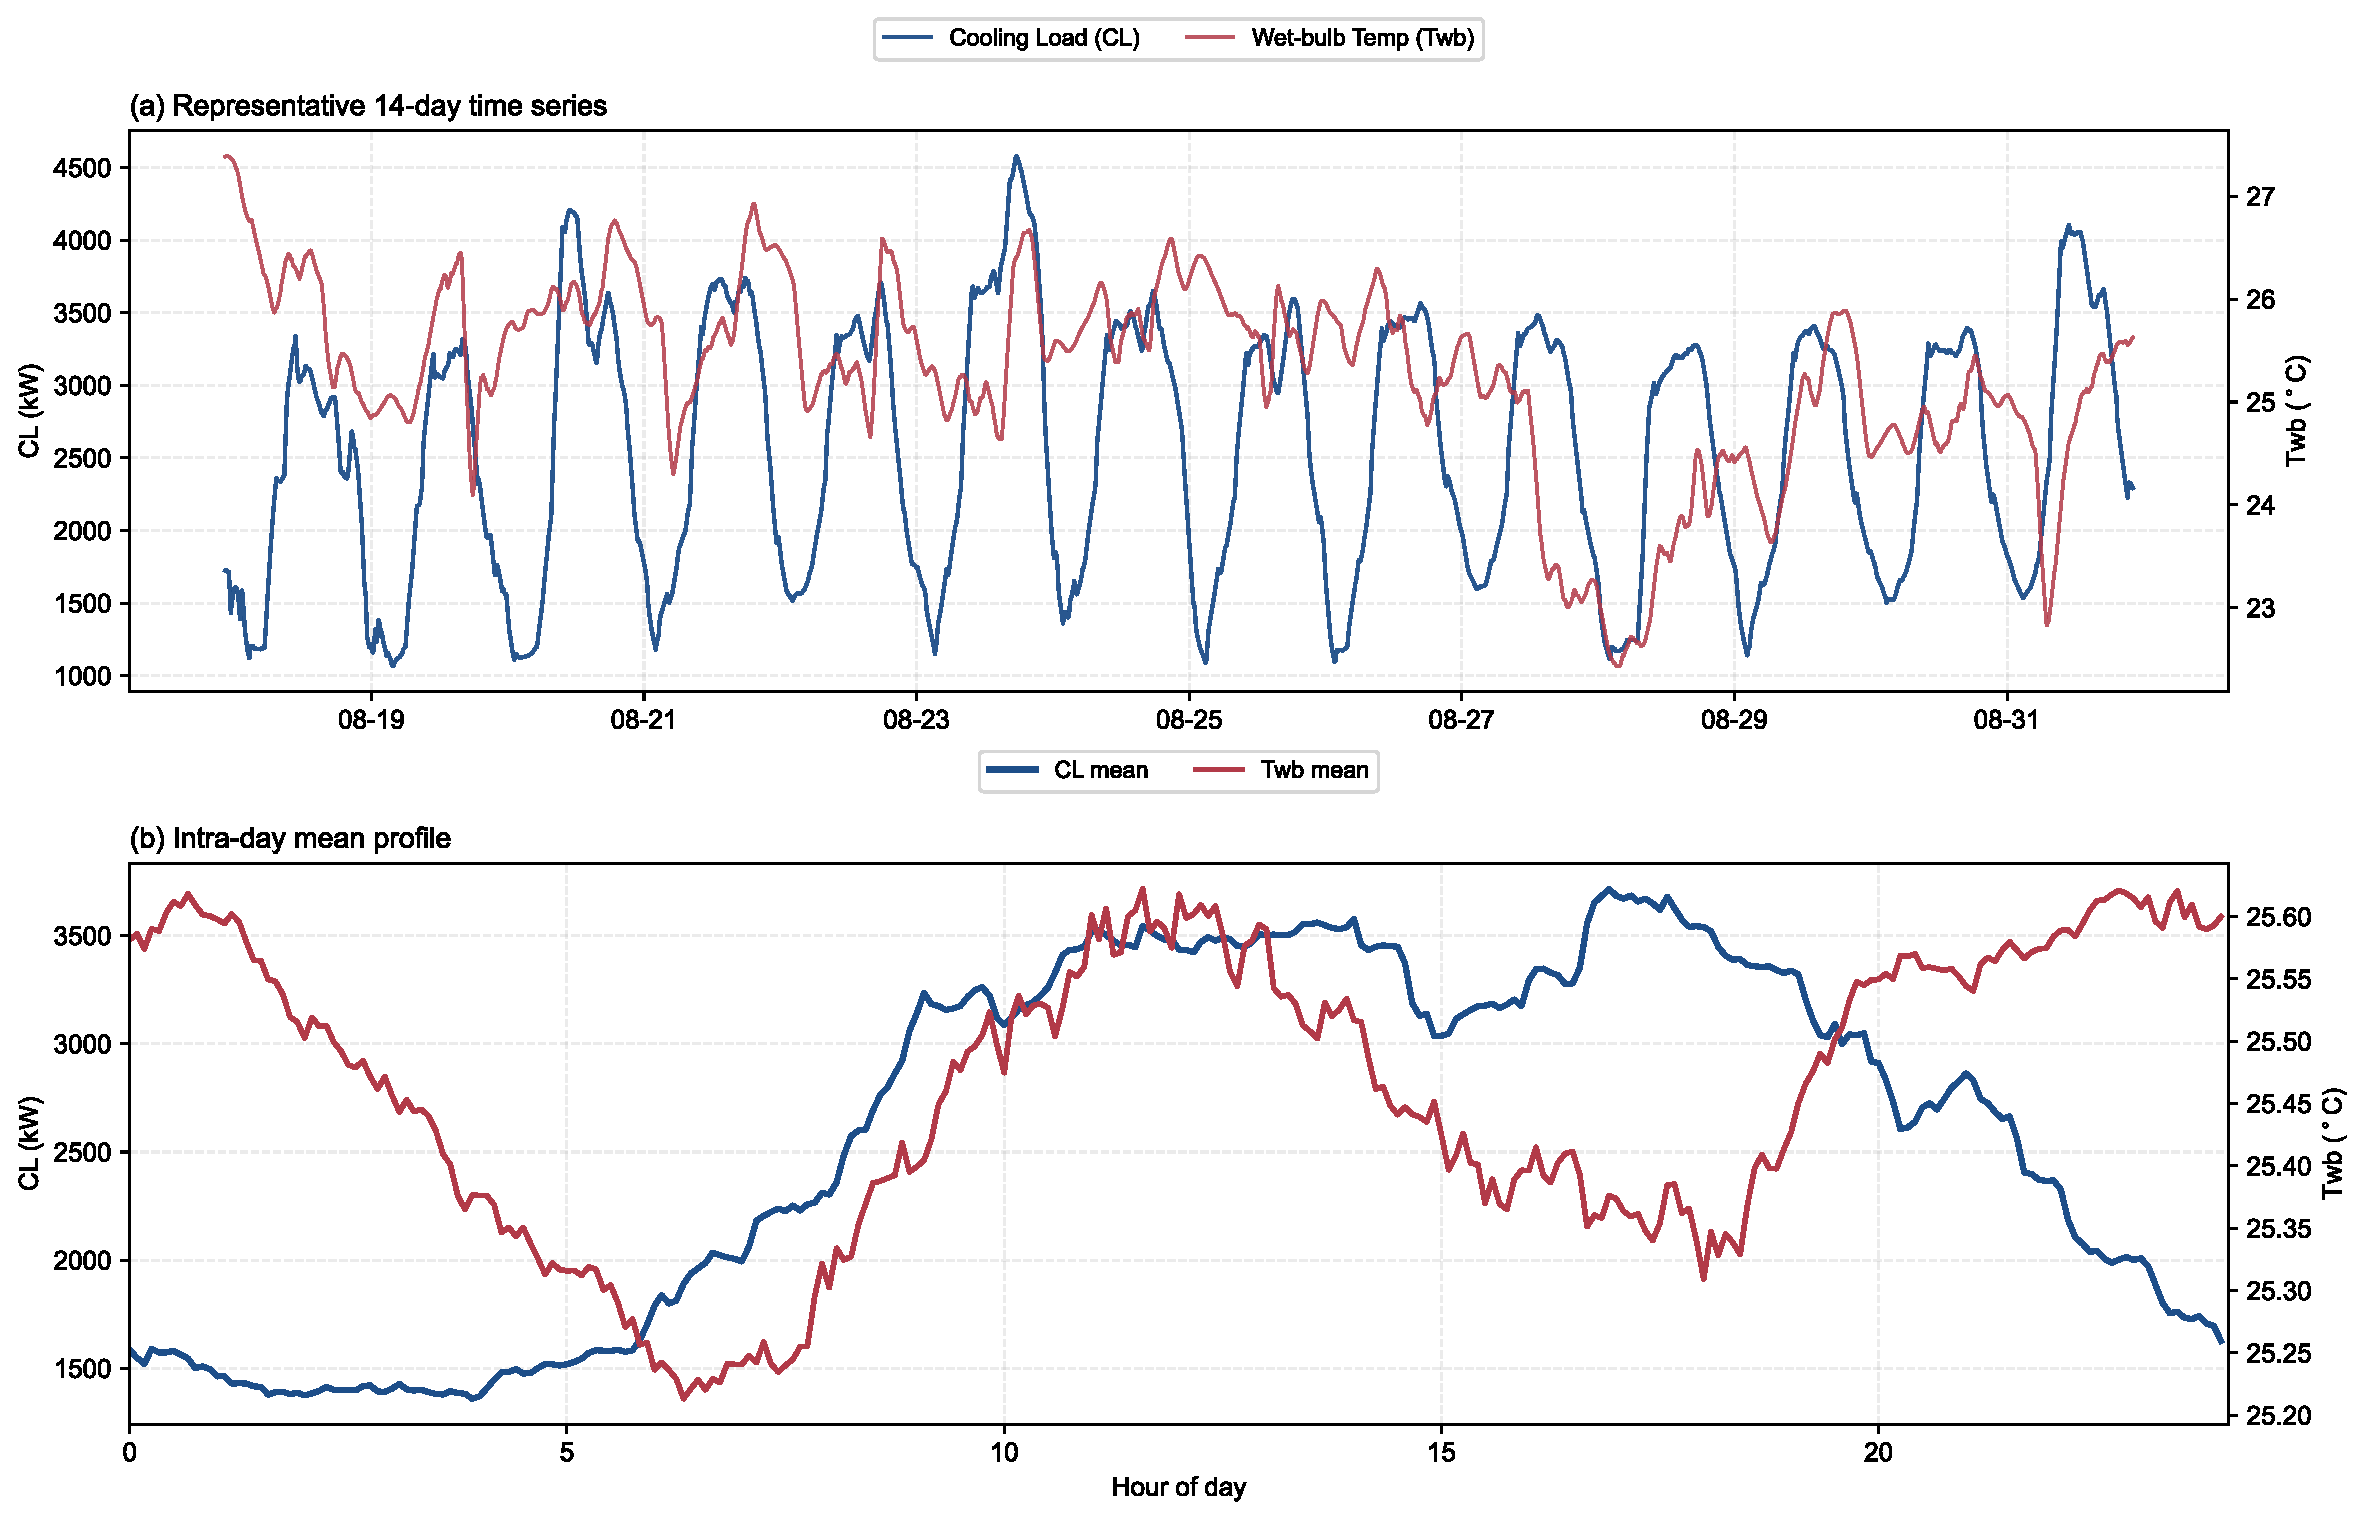
\includegraphics[width=\linewidth]{fig3_dataset_temporal_characteristics.pdf}}
\caption{Visualization of dataset temporal characteristics, full period sequence and intraday statistical profiles}\label{fig:dataset-temporal-characteristics}
\end{figure}

Figure~\ref{fig:dataset-distribution-dependence} further presents the marginal and joint distributions of the key variables. The cooling load \(Q_{\mathrm{load}}\) forms pronounced density clusters across multiple load ranges, indicating that the dataset contains several typical operating regimes, whereas \(T_{\mathrm{wb}}\) is concentrated within a relatively narrow range, indicating limited variability in the outdoor wet-bulb temperature in this dataset. Moreover, the joint density of \(T_{\mathrm{wb}}\) and \(Q_{\mathrm{load}}\) does not indicate a simple linear relationship. Instead, it forms several density clusters across different temperature ranges, indicating segmented distributional patterns and nonlinear joint variation between the two variables. Together with the temporal results in Figure~\ref{fig:dataset-temporal-characteristics}, these observations show that the dataset contains both intraday periodic load variation and nonlinear dependence among variables. These characteristics support adaptive triggering decisions by the streaming gating module based on the joint variation of cooling load and wet-bulb temperature rather than on deviations of a single variable.

\begin{figure}
\centering
\pandocbounded{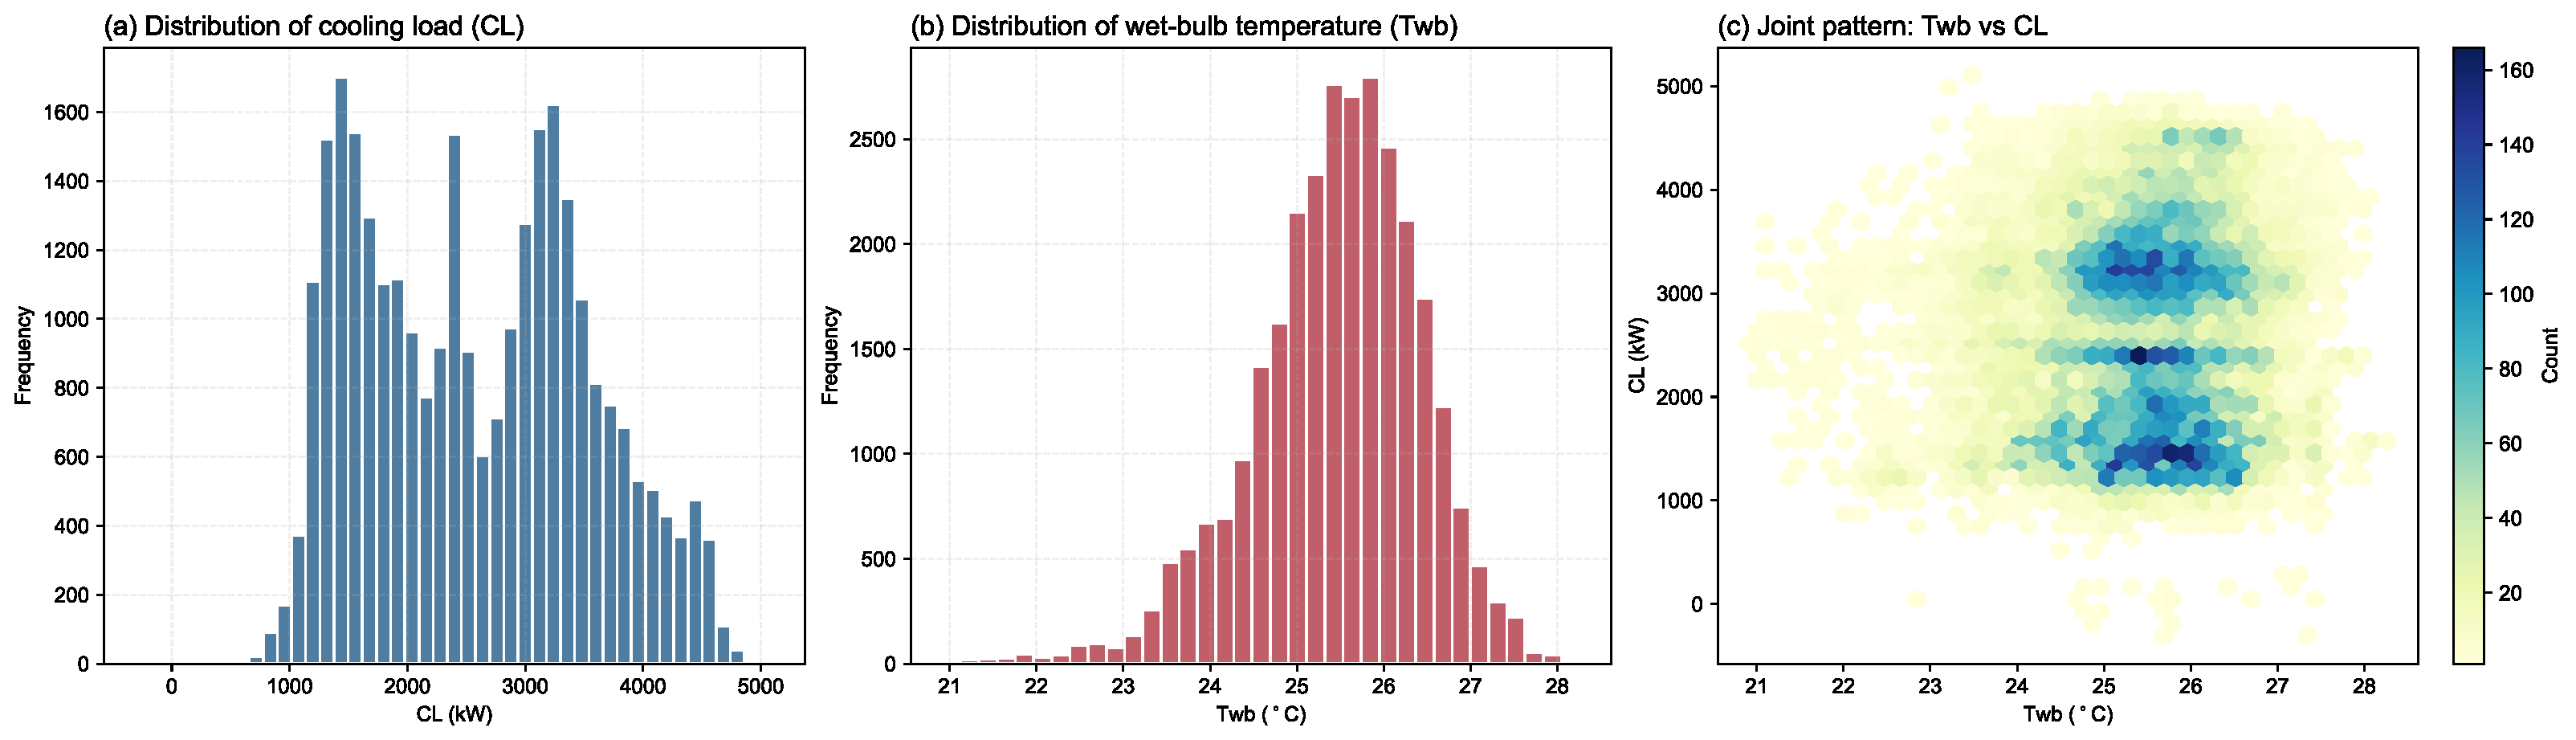
\includegraphics[width=\linewidth]{fig4_dataset_distribution_and_correlation.pdf}}
\caption{Visualization of dataset distributions and feature dependence}\label{fig:dataset-distribution-dependence}
\end{figure}

During preprocessing, the original collected cooling load sequence contained eight negative cooling load samples, which we truncated to zero. Because these samples account for only a negligible proportion of the full sequence, this correction has an insignificant effect on the overall load distribution. To introduce short-term predictive information, we use the one-step-ahead load prediction \(\hat{Q}_{\mathrm{load}}^{t+1}\) generated by the LSTM as an additional state input to characterize short-term load variation trends, thereby ensuring that the final state input includes both the current operating conditions and the short-term evolution trend.

To avoid temporal information leakage and better reflect practical online deployment conditions, we adopt a strict chronological splitting strategy. The dataset is divided into training, validation, and test sets in a ratio of 70:15:15. The normalization statistics, LSTM training, and hyperparameter selection are determined using only information from the training and validation sets, and they remain fixed during testing.

\section{Experiments and Results}\label{experiments-and-results}

\subsection{Experimental Setup}\label{experimental-setup}

\subsubsection{Experimental and Hyperparameter Settings}\label{experimental-and-hyperparameter-settings}

This section describes the experimental settings and hyperparameters. To ensure experimental reproducibility, the key parameters of the DQN-based control policy and the online streaming gate are kept constant across all experimental groups. Unless otherwise stated, the sampling interval is 5 min. All hyperparameters are determined through Bayesian optimization and fixed after validation set screening. Parameters of the DQN-based control policy define the state representation, action space, and training process of the reinforcement learning controller, whereas parameters of the online streaming gate govern the sensitivity and stability of event-driven action updates. The complete hyperparameter settings are reported in Table A.2 in Appendix A.

\subsubsection{Comparison Methods}\label{comparison-methods}

To systematically evaluate the control performance of the proposed ET-PRL method, we design six comparison strategies under the same test set and evaluation protocol, including two conventional control baselines and four RL strategies, to examine the relationship between control sparsity and energy efficiency under different triggering mechanisms.

The two conventional control baselines are PID and RBC. PID is a discrete closed-loop controller based on the supply water temperature error and adjusts the setpoint according to the current temperature deviation. RBC uses a fixed supply water temperature setpoint and serves as a rule-based baseline without learning.

All four RL strategies reuse the same trained DQN policy network and state inputs but differ in action update scheduling. Time-Triggered Reinforcement Learning (TTC-RL) includes TTC-RL-1 and TTC-RL-2. TTC-RL-1 recomputes and executes the control action at every sampling step, serving as the fixed-step RL baseline for the RL strategy group. TTC-RL-2 updates the action every two sampling steps, which allows us to examine the effect of fixed-frequency reduction. Static-Threshold Event-Triggered Control (ST-ETC) releases action updates only when the static threshold condition is satisfied, representing sparse control under a static trigger threshold. The proposed ET-PRL method incorporates streaming multi-scale anomaly scoring with a two-layer adaptive threshold, and triggers action updates only when the current operating condition deviates significantly from the recent reference distribution.

\subsubsection{Evaluation Metrics}\label{evaluation-metrics}

To comprehensively evaluate the performance of the proposed ET-PRL method, we construct four groups of evaluation metrics, namely energy efficiency, temperature control and stability, control sparsity, and execution-level statistics, to ensure the completeness and reproducibility of the experimental results.

\par\medskip
\noindent\textit{1. Energy efficiency metrics.}\label{energy-efficiency-metrics}
\par\smallskip

Energy efficiency is a core optimization objective in building energy management. We use the operating power of the chiller as the primary measurement target.

\par\smallskip
\noindent (1) Average daily energy consumption.
\par\nobreak Average daily energy consumption characterizes the average daily electricity use over the test period in kWh/day, as defined in Eq.~\eqref{eq:daily-energy}:

\[
E_{\text{daily}} = \frac{1}{D} \sum_{d=1}^{D} \left( \sum_{t=1}^{T_d} P_{\text{chiller}}(t) \cdot \Delta t \right) \tag{25}\label{eq:daily-energy}
\]

\noindent where \(D\) is the number of test days, \(T_d\) is the number of time steps on day \(d\), \(\Delta t\) is the sampling interval in hours, and \(P_{\text{chiller}}(t)\) is the chiller operating power at time step \(t\) in kW.

\par\smallskip
\noindent (2) Relative energy saving rate.
\par\nobreak Relative energy saving rate quantifies the energy saving effect of each evaluated method relative to the common baseline, as defined in Eq.~\eqref{eq:energy-saving-rate}:

\[
\eta_{\text{saving}}^{(i)} = \frac{E_{\text{base}} - E_{i}}{E_{\text{base}}} \times 100\% \tag{26}\label{eq:energy-saving-rate}
\]

\noindent where \(E_{\text{base}}\) is the cumulative energy consumption of the common baseline, and \(E_i\) is the cumulative energy consumption of the \(i\)th method.

\par\smallskip
\noindent (3) Average chiller power.
\par\nobreak Average chiller power reflects the average load level and operating intensity over the whole test period, as defined in Eq.~\eqref{eq:average-chiller-power}:

\[
\bar{P}_{\text{chiller}} = \frac{1}{N} \sum_{t=1}^{N} P_{\text{chiller}}(t) \tag{27}\label{eq:average-chiller-power}
\]

\noindent where \(N\) is the total number of test steps. This metric is physically related to \(E_{\text{daily}}\), but the two metrics characterize average load intensity and cumulative energy consumption, respectively.

\par\medskip
\noindent\textit{2. Temperature control and stability metrics.}\label{temperature-control-and-stability-metrics}
\par\smallskip

We use the chilled water supply temperature as the controlled variable, with the acceptable range set from \(15.0^\circ\mathrm{C}\) to \(19.0^\circ\mathrm{C}\).

\par\smallskip
\noindent (1) Performance preservation rate.
\par\nobreak Performance preservation rate (PPR) measures how well the event-driven mechanism preserves the cumulative reward of the fixed-step dense control baseline under sparse actuation, as defined in Eq.~\eqref{eq:ppr}:

\[
\mathrm{PPR} = \frac{R_{\text{event}}}{R_{\text{dense}}} \times 100\% \tag{28}\label{eq:ppr}
\]

\noindent where \(R_{\text{event}}\) and \(R_{\text{dense}}\) are the cumulative rewards of the event-driven strategy and the fixed-step dense control strategy over the same test period.

\par\smallskip
\noindent (2) Action smoothness.
\par\nobreak Action smoothness quantifies the impact intensity imposed on the actuator and is defined as the mean absolute change between adjacent control actions, as shown in Eq.~\eqref{eq:action-smoothness}:

\[
\bar{\Delta a} = \frac{1}{N-1} \sum_{t=1}^{N-1} |a_{t+1} - a_t| \tag{29}\label{eq:action-smoothness}
\]

A smaller value indicates smoother control actions and a lower risk of actuator oscillation.

\par\medskip
\noindent\textit{3. Control sparsity metrics.}\label{control-sparsity-metrics}
\par\smallskip

This group of metrics quantifies how effectively the event-driven mechanism reduces communication load and actuator wear.

\par\smallskip
\noindent (1) Total action updates.
\par\nobreak Total action updates count the number of actual control action changes during the test period, as defined in Eq.~\eqref{eq:action-updates}:

\[
N_{\text{update}} = \sum_{t=2}^{N} \mathbb{I}(a_t \neq a_{t-1}) \tag{30}\label{eq:action-updates}
\]

\noindent where \(\mathbb{I}(\cdot)\) is the indicator function. Under the fixed-step strategy, \(N_{\text{update}}\) is typically close to \(N\), whereas under the event-driven strategy, \(N_{\text{update}}\) is typically much smaller than \(N\).

\par\smallskip
\noindent (2) Daily trigger count.
\par\nobreak Daily trigger count is a physical measure of control frequency and reflects the average number of control actions executed per day, as defined in Eq.~\eqref{eq:daily-trigger-count}:

\[
N_{\text{daily}} = \frac{N_{\text{update}}}{D} \tag{31}\label{eq:daily-trigger-count}
\]

This metric directly reflects actuator wear risk through the actual number of control actions executed per day.

\par\smallskip
\noindent (3) Actuation compression ratio.
\par\nobreak Actuation compression ratio (ACR) measures the ratio of action updates between the fixed-step strategy and the evaluated strategy, as defined in Eq.~\eqref{eq:actuation-compression-ratio}:

\[
\mathrm{ACR} = \frac{N_{\text{fixed}}}{N_{\text{update}}} \tag{32}\label{eq:actuation-compression-ratio}
\]

\noindent where \(N_{\text{fixed}}\) and \(N_{\text{update}}\) are the total numbers of action updates under the fixed-step strategy and the evaluated strategy, respectively. A larger ACR indicates a stronger sparsification effect of the event-driven mechanism on control actions.

\par\smallskip
\noindent (4) Action reduction rate.
\par\nobreak Action reduction rate (ARR) measures the proportion of action updates reduced by the evaluated strategy relative to the fixed-step strategy, as defined in Eq.~\eqref{eq:action-reduction-rate}:

\[
\mathrm{ARR}=\left(1-\frac{N_{\text{update}}}{N_{\text{fixed}}}\right)\times 100\% = \left(1-\frac{1}{\mathrm{ACR}}\right)\times 100\% \tag{33}\label{eq:action-reduction-rate}
\]

A larger ARR indicates more effective compression of action updates and facilitates engineering interpretation and comparison across methods.

\par\medskip
\noindent\textit{4. Execution-level statistics.}\label{execution-level-statistics}
\par\smallskip

To characterize the operating behavior of the gate mechanism and the execution cost of the strategy, we further report the following execution-level statistics.

\par\smallskip
\noindent (1) Cumulative test reward.
\par\nobreak Cumulative test reward measures the overall control benefit accumulated during the test period, as defined in Eq.~\eqref{eq:cumulative-test-reward}:

\[
R_{\text{test}} = \sum_{t=1}^{N} r_t \quad \tag{34}\label{eq:cumulative-test-reward}
\]

\par\smallskip
\noindent (2) Average reward per update.
\par\nobreak Average reward per update measures the average control benefit per unit action update cost, as defined in Eq.~\eqref{eq:reward-per-update}:

\[
\bar{R}_{\text{update}} = \frac{R_{\text{test}}}{N_{\text{update}}} = \frac{\sum_{t=1}^{N} r_t}{N_{\text{update}}} \tag{35}\label{eq:reward-per-update}
\]

\noindent where \(N_{\text{update}}\) is the number of actual action updates. Under the fixed-step strategy, \(N_{\text{update}} = N\), whereas under the event-driven strategy, \(N_{\text{update}}\) is usually much smaller than \(N\).

\par\smallskip
\noindent (3) Trigger interval.
\par\nobreak Trigger interval measures the actual sparsity with which the gating layer releases action updates, as defined in Eq.~\eqref{eq:trigger-interval}:

\[
L_{\text{trigger}} = \frac{1}{K-1}\sum_{k=2}^{K}(t_k - t_{k-1}) \tag{36}\label{eq:trigger-interval}
\]

\noindent where \(t_k\) denotes the time step of the \(k\)th event trigger and \(K\) is the total number of triggers in the test trajectory. The trigger interval is an observed statistic from the test trajectory and differs from the minimum trigger interval constraint parameter \(\Delta_{\min}\) used in the gating mechanism.

\par\smallskip
\noindent (4) Hold length.
\par\nobreak Hold length measures setpoint stability at the execution layer, as defined in Eq.~\eqref{eq:hold-length}:

\[
L_{\text{hold}} = \frac{1}{M}\sum_{m=1}^{M}h_m \quad \tag{37}\label{eq:hold-length}
\]

\noindent where \(h_m\) denotes the length of the \(m\)th constant setpoint segment and \(M\) is the total number of holding segments in the test trajectory.

The evaluation metrics and optimization objectives are summarized in Table A.3 in Appendix A.

\subsection{Experimental Results Analysis}\label{experimental-results-analysis}

\paragraph{(1) Overall Performance Analysis}\label{overall-performance-analysis}

Based on the six comparison strategies and the related evaluation metrics, this section presents a comprehensive comparison of energy efficiency, temperature control, control sparsity, and execution-level performance across all strategies on the unified test set. Table 1 summarizes the test results of all strategies across all evaluation metrics.

\begin{table}[htbp]
\centering
\caption{Overall comparison results of multiple control strategies}\label{tab:overall-comparison}
\small
\setlength{\tabcolsep}{3pt}
\renewcommand{\arraystretch}{1.15}
\resizebox{\textwidth}{!}{%
\begin{tabular}{@{}lrrrrrrrrr@{}}
\toprule
\textbf{Strategy} &
\begin{tabular}[c]{@{}c@{}}\textbf{\(E_{\text{daily}}\)}\\\textbf{(kWh/day)}\end{tabular} &
\begin{tabular}[c]{@{}c@{}}\textbf{\(\eta_{\text{saving}}\)}\\\textbf{(\%)}\end{tabular} &
\begin{tabular}[c]{@{}c@{}}\textbf{\(\bar{P}_{\text{chiller}}\)}\\\textbf{(kW)}\end{tabular} &
\textbf{\(N_{\text{update}}\)} &
\begin{tabular}[c]{@{}c@{}}\textbf{ARR}\\\textbf{(\%)}\end{tabular} &
\textbf{\(\bar{\Delta a}\)} &
\textbf{\(R_{\text{test}}\)} &
\textbf{\(\bar{R}_{\text{update}}\)} &
\begin{tabular}[c]{@{}c@{}}\textbf{PPR}\\\textbf{(\%)}\end{tabular} \\
\midrule
PID & 8486.90 & -13.29 & 353.62 & - & - & - & - & - & - \\
RBC & 8548.72 & -14.12 & 356.20 & - & - & - & - & - & - \\
TTC-RL-1 & 7491.14 & - & 312.13 & 4404 & - & 0.8101 & \textbf{2054.63} & 0.4665 & - \\
TTC-RL-2 & 7489.98 & 0.02 & 312.08 & 2202 & 50.00 & \textbf{0.5617} & 2022.76 & 0.9186 & 98.45 \\
ST-ETC & 7485.44 & 0.08 & 311.89 & 3525 & 19.96 & 0.7711 & 2052.42 & 0.5822 & \textbf{99.89} \\
\textbf{ET-PRL} & \textbf{7331.85} & \textbf{2.13} & \textbf{305.49} & \textbf{2046} & \textbf{53.54} & 0.6014 & 1939.74 & \textbf{0.9481} & 94.41 \\
\bottomrule
\end{tabular}%
}
\end{table}

As shown in Table~\ref{tab:overall-comparison}, compared with the conventional control strategies, PID and RBC yield daily energy consumption values of 8486.90 and 8548.72 kWh/day, respectively, both of which are higher than the maximum value of 7491.14 kWh/day achieved by the RL strategies. ET-PRL obtains the lowest daily energy consumption at 7331.85 kWh/day, reducing daily energy consumption by 1155.05 and 1216.87 kWh/day relative to PID and RBC, corresponding to reductions of 13.61\% and 14.24\%, respectively. In terms of power, ET-PRL also achieves a lower average chiller power, with \(\bar{P}_{\text{chiller}}=305.49\,\mathrm{kW}\), compared with 353.62 kW for PID and 356.20 kW for RBC. These results show that, on this test set, ET-PRL regulates the cooling source system with lower daily energy consumption and lower average chiller power than the two conventional control strategies.

Within the RL strategy group evaluated against the common TTC-RL-1 baseline, ET-PRL achieves both higher sparsity and lower energy consumption. Specifically, TTC-RL-2 reduces the total number of action updates from 4404 to 2202, with an ARR of 50.00\%, but its relative energy saving rate is only 0.02\%, while ST-ETC obtains an ARR of 19.96\% and a relative energy saving rate of 0.08\%. In contrast, ET-PRL reduces the total number of action updates to 2046, reaches an ARR of 53.54\%, and increases the relative energy saving rate to 2.13\%. Normalized over the test period, the \(N_{\text{daily}}\) values of TTC-RL-1, TTC-RL-2, ST-ETC, and ET-PRL are 288.00, 144.00, 230.51, and 133.80 updates per day, respectively. Their corresponding ACR values are 1.0000, 2.0000, 1.2494, and 2.1525. These results indicate that the advantage of ET-PRL does not simply come from lowering the action update frequency. Instead, it comes from more accurate trigger timing: the method tends to update actions when load or operating condition changes require control adjustment, while holding the previous action during relatively stable periods.

In terms of action smoothness, ET-PRL obtains \(\bar{\Delta a}=0.6014\), which is 25.76\% lower than the 0.8101 of TTC-RL-1 and 22.01\% lower than the 0.7711 of ST-ETC. This indicates that ET-PRL reduces large setpoint changes between adjacent time steps. This value is slightly higher than the 0.5617 of TTC-RL-2, suggesting that ET-PRL does not simply minimize action variation but reduces high-frequency control fluctuations while retaining a moderate level of action adjustment.

For the reward, cumulative return and return per update should be interpreted separately. ET-PRL obtains a cumulative test reward \(R_{\text{test}}\) of 1939.74, which is lower than the 2054.63 of TTC-RL-1 and corresponds to a PPR of 94.41\%. However, its average reward per update \(\bar{R}_{\text{update}}\) reaches 0.9481, the highest value among the RL strategies. This represents an improvement of approximately 103.24\% over the 0.4665 of TTC-RL-1 and approximately 62.85\% over the 0.5822 of ST-ETC, and it also exceeds the 0.9186 of TTC-RL-2. These results suggest that although ET-PRL reduces the number of action updates, the remaining updates occur more often during periods when load or operating condition changes require control adjustment. As a result, it improves update efficiency while retaining most of the cumulative reward, which is consistent with the design objective of event-driven control for intervention on demand.

\paragraph{(2) Chilled Water Supply Temperature Setpoint Strategy Behavior Analysis}\label{chilled-water-supply-temperature-setpoint-strategy-behavior-analysis}

To further examine whether different trigger mechanisms affect the preference for selecting the chilled water supply temperature setpoint, Figure~\ref{fig:t-chws-macro-distribution} compares the overall action distributions of each strategy over the discrete action space of \(T_{\mathrm{chws}}\). It should be noted that ST-ETC reaches an action equivalence ratio of 99.2\% relative to TTC-RL-1, indicating that the setpoints selected by the two strategies are almost identical at most time steps. This suggests that the main function of ST-ETC is to reduce the action update frequency of TTC-RL-1, rather than to substantially change the setpoint selection preference learned by the original Q network. Therefore, Figure~\ref{fig:t-chws-macro-distribution} presents the action distributions of TTC-RL-1 and ST-ETC jointly as the reference, which will highlight how ET-PRL adjusts the action selection distribution later.

\begin{figure}
\centering
\pandocbounded{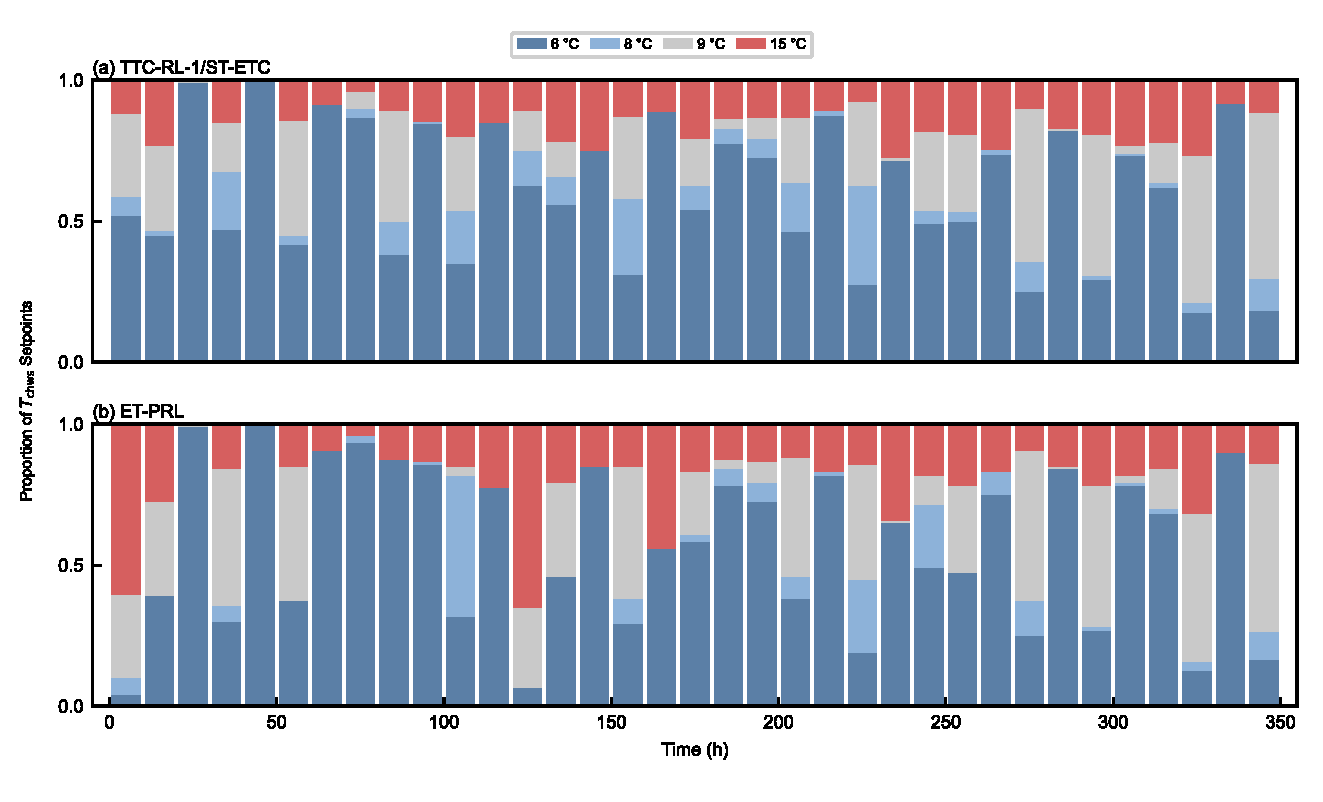
\includegraphics[width=\linewidth]{fig6_t_chws_macro_distribution.pdf}}
\caption{Comparison of the \(T_{\mathrm{chws}}\) window distributions for ET-PRL, TTC-RL-1, and ST-ETC. Each bar represents the action proportion within a 10 h window}\label{fig:t-chws-macro-distribution}
\end{figure}

Figure~\ref{fig:t-chws-macro-distribution} shows that, during typical low-load periods such as 0 to 50 h and 200 to 250 h, ET-PRL substantially increases the proportion of high-temperature setpoints such as 15~$^\circ$C. This behavior is consistent with the off-design thermodynamic characteristics of chillers. When the building cooling demand is weak, increasing \(T_{\mathrm{chws}}\) is equivalent to increasing the evaporation temperature, which reduces the compressor pressure ratio and improves COP, thereby reducing electricity consumption per unit cooling output without violating indoor thermal comfort limits. It should be emphasized that ST-ETC and ET-PRL reuse the same trained TTC-RL-1 Q network and the same state inputs, so both strategies retain value estimation capability based on predictive features. Their difference mainly lies in the gating layer. The static threshold in ST-ETC is more likely to mismatch the current operating condition under cross-period distribution shift, which can cause false triggering at noncritical moments and shorten the continuous holding duration of efficient setpoints. In contrast, the streaming local-global two-layer adaptive threshold in ET-PRL can correct the trigger boundary online and filter high-frequency noise-induced triggers, allowing high-temperature setpoints to be held for longer continuous periods and leading to a clearer adjustment of the action selection distribution.

However, the overall window distribution alone is insufficient to explain how the action selection distribution changes. On the one hand, setpoint holding and updating behaviors should be examined in representative temporal segments during load variation. On the other hand, the degree of action deviation between event-triggered strategies and TTC-RL-1 should be quantified over the full sample, so that we can determine whether these strategies form setpoint adjustments that are genuinely distinct from the baseline. For this reason, Figure~\ref{fig:t-chws-delta-analysis} further analyzes the trigger behavior of ET-PRL from two perspectives, namely local trajectory response and global difference frequency.

\begin{figure}[!htbp]
\centering
\pandocbounded{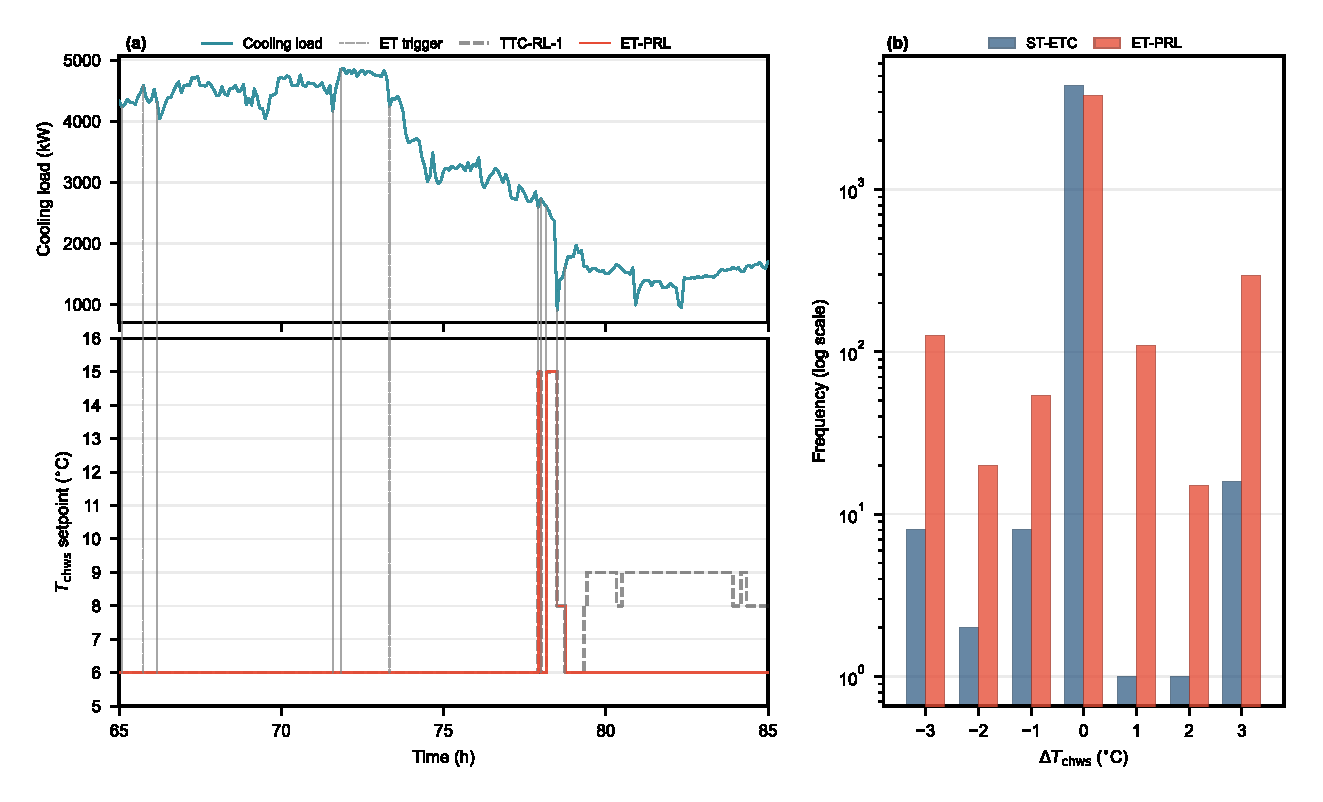
\includegraphics[width=0.88\linewidth]{fig7_t_chws_delta_analysis.pdf}}
\caption{Local event-triggered response and global difference frequency statistics. Panel a shows the cooling load and absolute setpoint trajectories from 65 h to 85 h, and panel b shows the logarithmic frequency distributions of \(\Delta T_{\mathrm{chws}}\) for ST-ETC and ET-PRL relative to TTC-RL-1}\label{fig:t-chws-delta-analysis}
\end{figure}

For the local trajectory analysis, panel a of Figure~\ref{fig:t-chws-delta-analysis} examines a representative window from 65 to 85 h. ET-PRL exhibits longer stepwise holding periods and updates the setpoint only when key disturbances occur, whereas TTC-RL-1 maintains high-frequency time-triggered updates. Because the same trained Q network is used, this difference mainly comes from when updates are triggered. ST-ETC is constrained by a static boundary and is therefore more likely to trigger falsely near the boundary, which causes frequent switching and drives the output closer to the baseline strategy. ET-PRL suppresses updates caused by noise through the local-global two-layer adaptive threshold and the minimum trigger interval, which allows the predictive Q network to keep efficient setpoints for longer periods during low-load windows.

At the global difference level, panel b of Figure~\ref{fig:t-chws-delta-analysis} shows that the proportion of nonzero differences between ST-ETC and TTC-RL-1 is only 0.82\%, whereas the corresponding proportion for ET-PRL is 14.12\%. The full sample variances of the differences are \(0.446\) and \(5.879\), respectively. This indicates that the action outputs of ST-ETC remain very close to the baseline strategy and are insufficient to produce substantive temperature setpoint optimization. In contrast, ET-PRL achieves clearer action selection adjustment while preserving sparse execution.

\paragraph{(3) Event-Triggered Control Sparsity and Temporal Dynamics Analysis}\label{event-triggered-control-sparsity-and-temporal-dynamics-analysis}

The above results show that ET-PRL not only reduces the action update frequency but also changes the distribution of chilled water supply temperature setpoints in the action space. To further characterize the temporal structure of control sparsity and the dynamic response of the system, we compare ET-PRL, ST-ETC, and TTC-RL-1 using the trigger interval and action holding length defined above. The trigger interval reflects the actual sparsity of trigger events at the gating layer, whereas the action holding length reflects setpoint stability at the execution layer. Even after a trigger occurs, the policy network may still output the same optimal setpoint as in the previous step, so the action holding length in the realized trajectory is usually greater than or equal to the trigger interval.

\begin{table}[htbp]
\centering
\caption{Temporal sparsity and action holding statistics of different control strategies}\label{tab:temporal-sparsity}
\small
\setlength{\tabcolsep}{8pt}
\renewcommand{\arraystretch}{1.15}
\resizebox{\textwidth}{!}{%
\begin{tabular}{@{}lrrrr@{}}
\toprule
\textbf{Strategy} &
\begin{tabular}[c]{@{}c@{}}\textbf{Mean Trigger}\\\textbf{Interval (steps)}\end{tabular} &
\begin{tabular}[c]{@{}c@{}}\textbf{Daily Trigger}\\\textbf{Count}\end{tabular} &
\begin{tabular}[c]{@{}c@{}}\textbf{Mean Holding}\\\textbf{Length (steps)}\end{tabular} &
\begin{tabular}[c]{@{}c@{}}\textbf{95th Percentile}\\\textbf{\(P_{95}\) (steps)}\end{tabular} \\
\midrule
TTC-RL-1 & 1.000 & 275.25 & 7.57 & 42.9 \\
ST-ETC & 1.249 & 220.31 & 7.89 & 43.3 \\
\textbf{ET-PRL} & \textbf{2.117} & \textbf{127.88} & \textbf{11.56} & \textbf{57.0} \\
\bottomrule
\end{tabular}%
}
\end{table}

Based on these statistics, the mean trigger interval of ET-PRL is 2.117 steps, which is much higher than 1.249 steps for ST-ETC and 1.000 step for TTC-RL-1, and the corresponding daily trigger counts are 127.88, 220.31, and 275.25, respectively. ET-PRL also achieves a longer mean action holding length of 11.56 steps, compared with 7.89 steps for ST-ETC and 7.57 steps for TTC-RL-1. Its distribution exhibits a pronounced long-tail pattern, with the 95th percentile \(P_{95}\) reaching 57.0 steps, or about 4.75 h, whereas the corresponding values for ST-ETC and TTC-RL-1 are only 43.3 and 42.9 steps. These results indicate that the dynamic threshold gating mechanism yields a lower control update frequency and longer holding durations during stable periods.

To further illustrate the distribution pattern of these trigger interval differences, Figure~\ref{fig:action-update-interval-distribution} shows the distribution of action update intervals under the different control strategies. The main panel reports the proportion in each interval bin for TTC-RL-1, ST-ETC, and ET-PRL, and the inset enlarges the long-tail region for intervals of at least 4 steps. TTC-RL-1 concentrates almost entirely at an interval of 1 step because it updates at a fixed cadence, whereas ST-ETC updates are mainly concentrated in the short-interval range. By contrast, ET-PRL exhibits a much more pronounced long-tail pattern, with a maximum trigger interval of 74 steps, indicating that the dynamic event gating mechanism can keep the setpoint unchanged for longer periods under low-disturbance conditions.

\begin{figure}[!htbp]
\centering
\pandocbounded{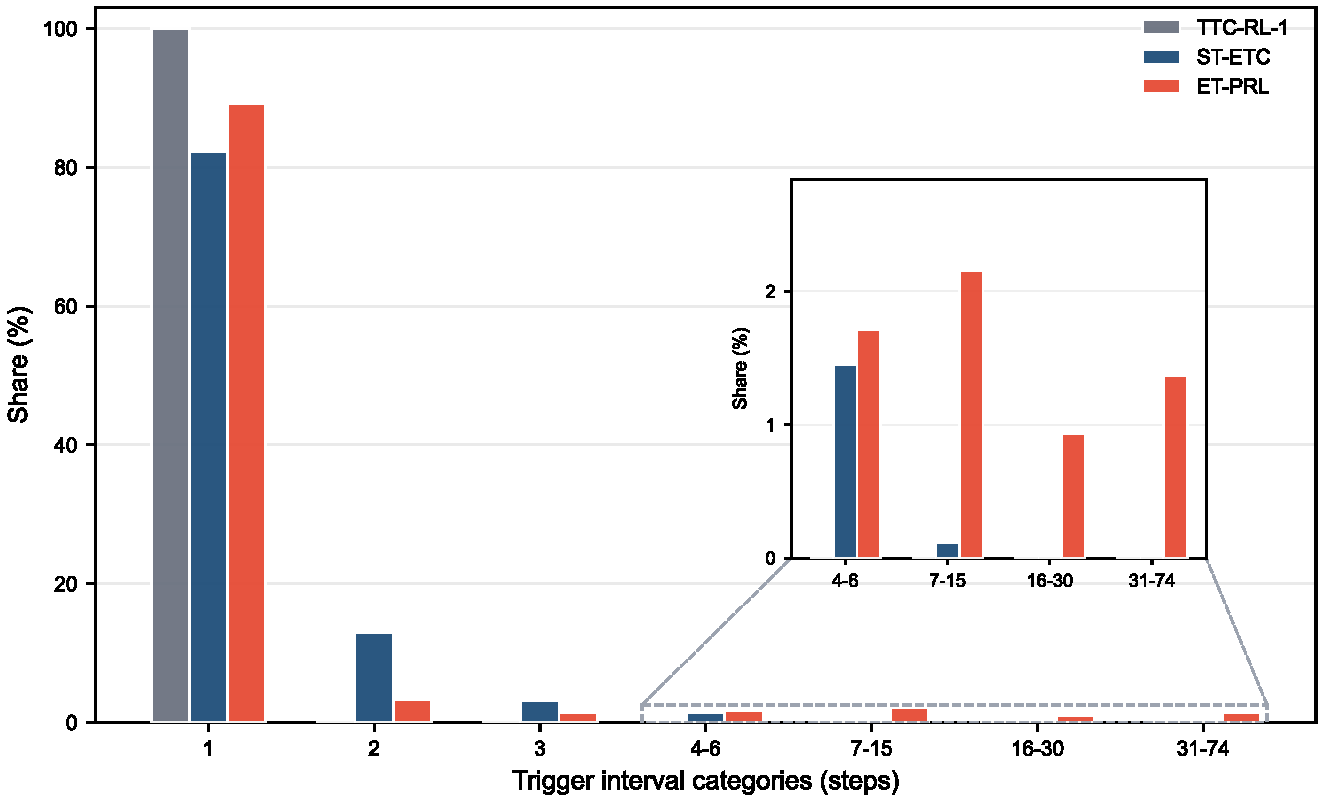
\includegraphics[width=0.9\linewidth]{fig8_action_update_interval_distribution.pdf}}
\caption{Distribution of action update intervals under different control strategies. The main panel shows the share of each discrete bin, and the inset enlarges the long-tail region}\label{fig:action-update-interval-distribution}
\end{figure}

To reveal the temporal alignment between dynamic load variation and triggering actions, Figure~\ref{fig:trigger-load-alignment} further presents the alignment results for a representative day 5 operating profile.

\begin{figure}[!htbp]
\centering
\pandocbounded{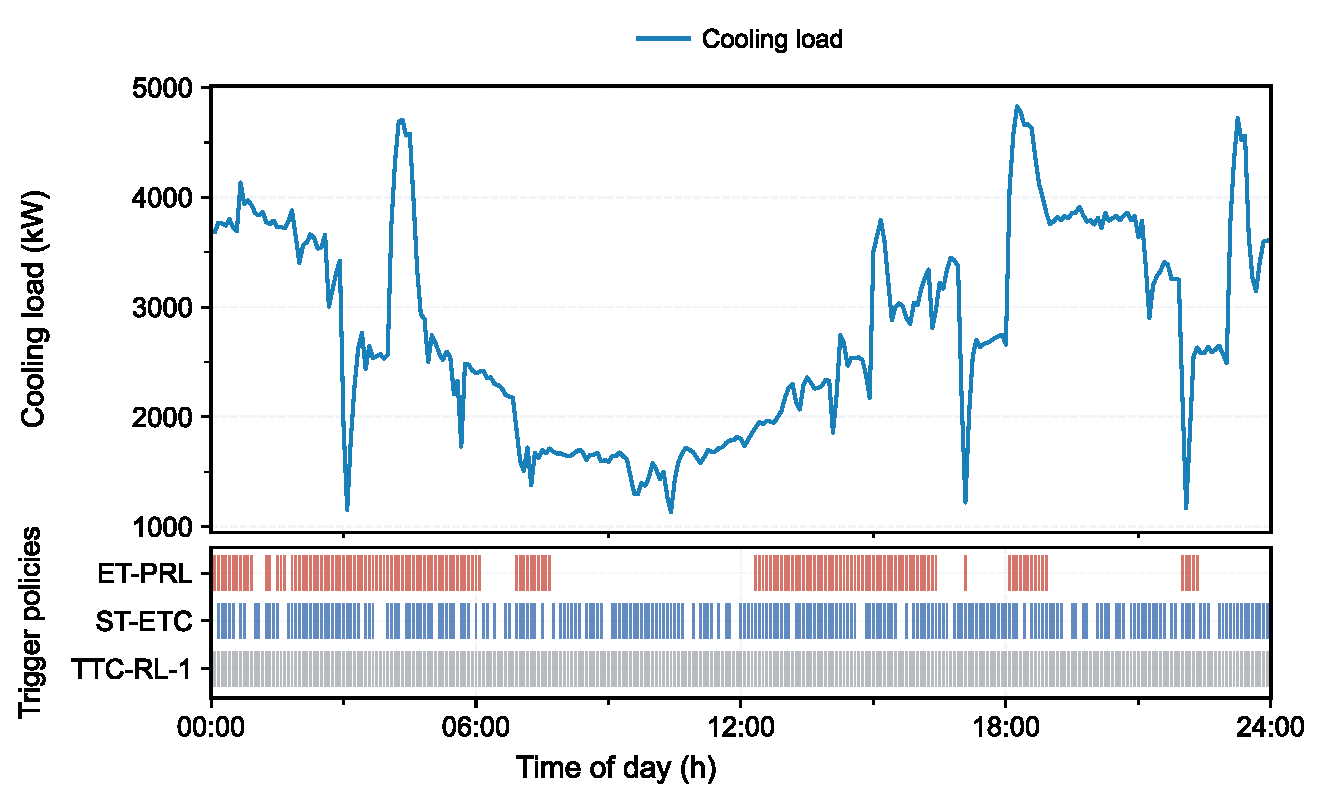
\includegraphics[width=0.9\linewidth]{fig9_trigger_load_alignment.pdf}}
\caption{Alignment of daily load variation and trigger times on day 5 with 5-min sampling. Panel a shows the cooling load curve, panel b shows the trigger pulse raster of ET-PRL, ST-ETC, and TTC-RL-1, and the shaded band across panels indicates a typical high-variation period}\label{fig:trigger-load-alignment}
\end{figure}

By comparison, the ET-PRL trigger pulses are densely distributed during load ramp-up and abrupt change periods, but become much sparser during stable periods such as nighttime. In contrast, because ST-ETC uses a fixed decision boundary, its trigger actions are more concentrated in time, whereas TTC-RL-1 triggers at every time step.

Across the full test set, we define the interval where the absolute cooling load variation exceeds the 85th percentile \(q_{85}\) of all samples as the high-variation region, and the interval below the 30th percentile \(q_{30}\) as the low-variation region, namely a relatively stable base-load period. The statistics show that the trigger rate of ET-PRL reaches 0.707 in the high-variation region and drops to 0.350 in the low-variation region, giving a ratio of 2.02. The corresponding ratios are 1.73 for ST-ETC and 1.00 for TTC-RL-1. To verify the robustness of this conclusion, we further relax the percentile thresholds. When the evaluation intervals are replaced by the 80th and 20th percentile pair or the 90th and 40th percentile pair, the high-to-low variation trigger rate ratio of ET-PRL remains stable at 1.91 and 2.02, respectively.

From an energy efficiency perspective, the benefits of control sparsification are reflected not only in reduced mechanical wear on the actuators, but also in the suppression of transient efficiency losses caused by frequent chiller adjustments. Conventional high-frequency feedback control with a fixed-step strategy forces centrifugal chillers to repeatedly enter non-steady transition stages, thereby moving away from the steady operating boundary associated with the optimal COP. In contrast, the long holding characteristic shown by ET-PRL provides the chiller with a much wider window for continuous steady operation. This working mode reduces both actuator mechanical wear and the extra energy loss caused by frequent chiller adjustments.

In summary, the proposed ET-PRL method exhibits an adaptive temporal pattern with fast responses during disturbed periods and fewer updates during stable periods. This pattern shows that multi-scale anomaly score fusion in the streaming gating mechanism can effectively capture disturbances at different timescales, while the local-global two-layer adaptive threshold helps suppress control oscillations near the threshold boundary. Together, these components provide a clear physical explanation for sparse control.

\paragraph{(4) Ablation Study Analysis}\label{ablation-study-analysis}

To quantify the contribution of each component in the proposed method, we conduct an ablation study under a controlled-variable experimental design. Unless otherwise specified, all experimental groups use the same training configuration, test set, and evaluation protocol. In addition to TTC-RL-1, the ablation study includes six comparison methods, consisting of five simplified variants and the full model, to analyze the contributions of the two-layer threshold module and the multi-scale module. Table~\ref{tab:key-module-ablation} summarizes the test-set results of all strategies, where relative metrics such as ACR and PPR use TTC-RL-1 as the computational baseline, whereas the remaining metrics are test-set statistics.

\begin{table}[htbp]
\centering
\caption{Key module ablation results}\label{tab:key-module-ablation}
\small
\setlength{\tabcolsep}{5pt}
\renewcommand{\arraystretch}{1.12}
\resizebox{\textwidth}{!}{%
\begin{tabular}{@{}lrrrrrr@{}}
\toprule
\textbf{Method} & \(R_{\text{test}}\) & \(N_{\text{update}}\) & \(N_{\text{daily}}\) &
\begin{tabular}[c]{@{}c@{}}\(E_{\text{daily}}\)\\kWh/day\end{tabular} & ACR & PPR \\
\midrule
TTC-RL-1 baseline & 2054.63 & 4404 & 288.00 & 7491.14 & 1.0000 & 100.00\% \\
Local Threshold Only & 1958.05 & 2257 & 147.60 & 7367.57 & 1.9513 & 95.30\% \\
Global Threshold Only & 1977.54 & 2251 & 147.20 & 7409.42 & 1.9565 & 96.25\% \\
Short-scale Only & 1951.74 & 2122 & 138.77 & 7407.03 & 2.0754 & 94.99\% \\
Medium-scale Only & 2041.96 & 3891 & 254.45 & 7484.70 & 1.1318 & 99.38\% \\
Long-scale Only & 2032.01 & 4334 & 283.42 & 7431.26 & 1.0162 & 98.90\% \\
\textbf{Full ET-PRL} & \textbf{1939.74} & \textbf{2046} & \textbf{133.80} & \textbf{7331.85} & \textbf{2.1525} & \textbf{94.41\%} \\
\bottomrule
\end{tabular}%
}
\end{table}

\begin{figure}[H]
\centering
\pandocbounded{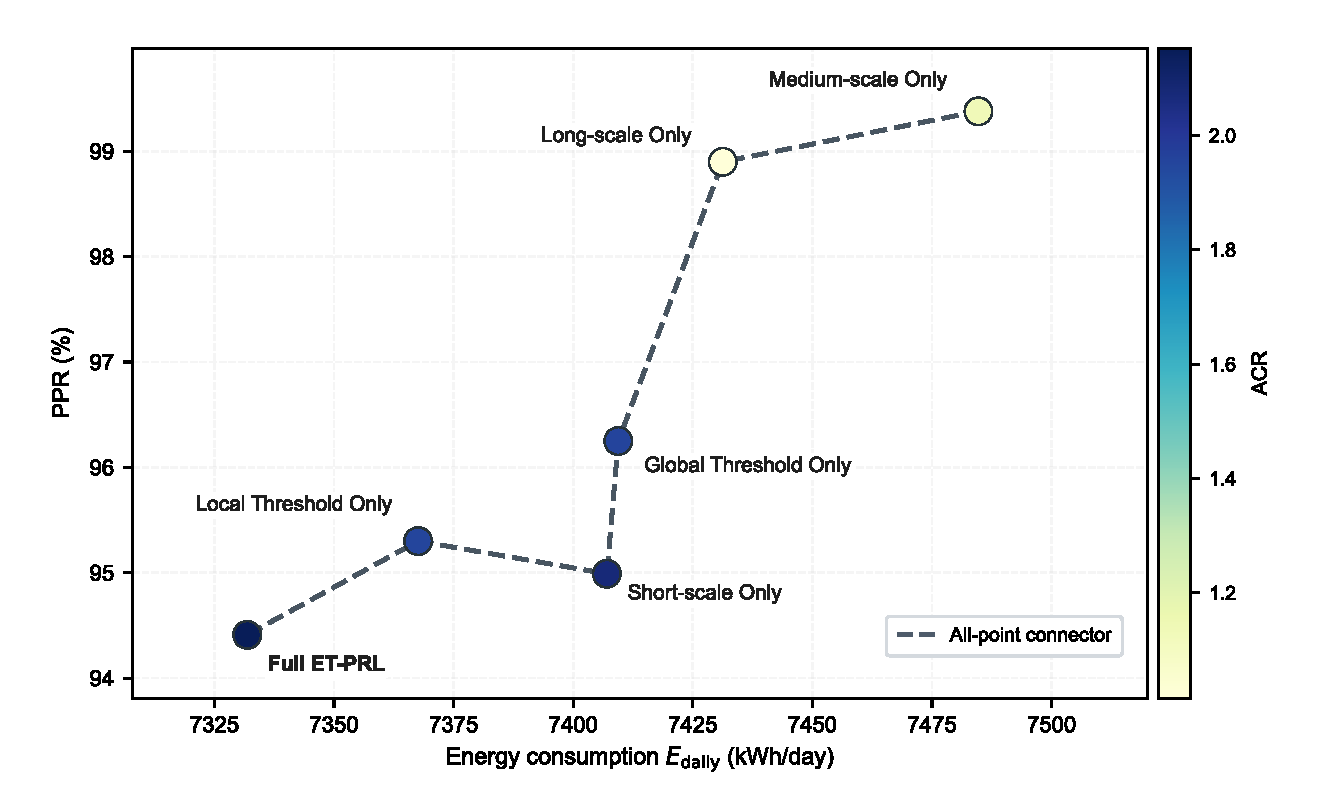
\includegraphics[width=0.78\linewidth]{fig10_ablation_pareto_scatter.pdf}}
\caption{Scatter plot of ablation strategies under the trade-off among energy consumption, performance, and sparsity. The x-axis indicates average daily energy consumption, the y-axis indicates PPR, color encodes ACR, and text labels identify each ablation strategy}\label{fig:ablation-tradeoff}
\end{figure}

As shown in Figure~\ref{fig:ablation-tradeoff}, under the three-objective trade-off that minimizes \(E_{\text{daily}}\) while maximizing PPR and ACR, Full ET-PRL lies in the low energy consumption and high sparsity region. It achieves the lowest \(E_{\text{daily}}\) and the highest ACR among the ablation groups while maintaining a PPR of 94.41\%, making it closer to the ideal compromise solution on the current test set.

For temporal-scale ablation, Short-scale Only yields a slightly higher PPR than Full ET-PRL, with values of 94.99\% and 94.41\%, respectively, but its ACR decreases by 3.58\% and its daily energy consumption increases by 75.18 kWh/day. Given the comfort constraints adopted in this study, both methods maintain PPR values above 94\%, and the difference of 0.58 percentage points is small. In contrast, the reduced action compression capability and increased energy consumption directly raise the execution burden and operating cost. Furthermore, although Medium-scale Only and Long-scale Only maintain high PPR values of 99.38\% and 98.90\%, respectively, their trigger sparsity deteriorates markedly, with \(N_{\text{daily}}\) values of 254.45 and 283.42, and their energy optimization remains limited, with daily energy consumption values of 7484.70 and 7431.26 kWh/day. These results indicate that single-scale statistics cannot simultaneously accommodate short-term disturbance response and long-term drift correction.

We use a compact three-dimensional state vector \(s_t = [Q_{\mathrm{load}}^t, T_{\mathrm{wb}}^t, \hat{Q}_{\mathrm{load}}^{t+1}]\) without stacking high-dimensional historical sequences. This design reduces online inference overhead but also requires the gating mechanism to compensate for long-term historical information. If the gate relies only on short-scale statistics, the gating score may treat slow drift as a new local steady state, weakening its ability to identify long-term energy efficiency degradation. Physically, during seasonal transitions, the equivalent thermal resistance and heat storage state of the building envelope change gradually, and long-term chiller operation may also lead to accumulated fouling thermal resistance in heat exchangers. These slowly changing factors progressively increase the effective cooling load required to achieve the same cooling effect. A short-scale gate may absorb this slow shift into the local steady baseline, causing the controller to keep the action unchanged when policy correction should be triggered. As a result, the control setpoint may stay for an extended period in a locally stable but overall suboptimal region, for example near a relatively high value of 15~$^\circ$C, while the chiller continues to operate away from the optimal COP condition, eventually leading to increased daily energy consumption. By introducing medium- and long-scale scores, Full ET-PRL supplements the compact state representation with implicit historical information and can identify gradual equipment performance degradation and seasonal drift as events that require intervention, which explains its lower daily energy consumption than Short-scale Only.

For the two-layer threshold ablation, Local Threshold Only and Global Threshold Only obtain ACR values of 1.9513 and 1.9565, respectively, both lower than the 2.1525 of Full ET-PRL. Their daily energy consumption values are 7367.57 and 7409.42 kWh/day, respectively, which are also higher than that of Full ET-PRL. Mechanistically, Local Threshold Only tends to overfollow recent changes, meaning that it is overly sensitive to short-term disturbances while lacking long-term baseline constraints. Global Threshold Only, by contrast, tends to show delayed response, meaning that it responds too slowly to minute-scale disturbances and therefore requires larger compensatory control afterward. These two simplified variants correspond to the loss of fast response capability and long-term steady-state constraint, respectively. With two-layer threshold coordination, Full ET-PRL obtains lower daily energy consumption and a higher ACR in Table~\ref{tab:key-module-ablation} while maintaining a PPR of 94.41\%.

\paragraph{(5) Parameter Sensitivity Analysis}\label{parameter-sensitivity-analysis}

To further show how streaming gate hyperparameters affect trigger count, reward, and daily energy consumption in the proposed ET-PRL method, we conduct single-factor parameter perturbation experiments. In each run, we adjust only one parameter, keep the remaining parameters at their baseline values, and evaluate \(R_{\text{test}}\), \(N_{\text{daily}}\), and \(E_{\text{daily}}\) on the same test set. The analyzed parameters are the quantile level \(q\), the bias correction term \(b_{\mathrm{bias}}\), the hysteresis margin \(m_{\mathrm{hys}}\), the local window length \(W\), and the short-scale weight \(w_s\).

\paragraph{\texorpdfstring{1. Quantile Level \(q\)}{1. Quantile Level q}}\label{quantile-level-q}

\begin{longtable}[]{@{}
  >{\centering\arraybackslash}p{(\linewidth - 6\tabcolsep) * \real{0.2500}}
  >{\centering\arraybackslash}p{(\linewidth - 6\tabcolsep) * \real{0.2500}}
  >{\centering\arraybackslash}p{(\linewidth - 6\tabcolsep) * \real{0.2500}}
  >{\centering\arraybackslash}p{(\linewidth - 6\tabcolsep) * \real{0.2500}}@{}}
\caption{Sensitivity results for quantile level \(q\)}\tabularnewline
\sensitivitytablehead{\(q\)}
\endfirsthead
\sensitivitytablehead{\(q\)}
\endhead
\bottomrule\noalign{}
\endlastfoot
0.55 & 1284.49 & 0.65 & 6921.91 \\
0.60 & 1103.87 & 0.78 & 6095.77 \\
0.65 & 1241.99 & 1.05 & 6146.26 \\
0.70 & 1325.45 & 1.50 & 6329.57 \\
0.75 & 1397.99 & 1.83 & 6632.52 \\
0.80 & 1531.77 & 2.29 & 7230.91 \\
0.85 & 1560.47 & 3.20 & 7097.17 \\
0.90 & 1678.75 & 5.43 & 7513.54 \\
\end{longtable}

The quantile level \(q\) mainly changes the trend in trigger frequency associated with the quantile reference. As shown in Table 4, when \(q\) increases from 0.60 to 0.90, \(N_{\text{daily}}\) increases from 0.78 to 5.43, \(R_{\text{test}}\) increases from 1103.87 to 1678.75, and \(E_{\text{daily}}\) also increases from 6095.77 kWh/day to 7513.54 kWh/day. Overall, a lower \(q\) leads to fewer gate triggers, insufficient action updates, and a lower reward, while energy consumption is also lower. A higher \(q\) increases the trigger count and makes the controller update setpoints more often, which improves reward but raises daily energy consumption. Therefore, increasing \(q\) mainly produces a simultaneous increase in reward and trigger count at the cost of higher daily energy consumption.

\paragraph{\texorpdfstring{2. Bias Correction Term \(b_{\mathrm{bias}}\)}{2. Bias Correction Term b\_\{\textbackslash mathrm\{bias\}\}}}\label{bias-correction-term-b_mathrmbias}

\begin{longtable}[]{@{}
  >{\centering\arraybackslash}p{(\linewidth - 6\tabcolsep) * \real{0.2500}}
  >{\centering\arraybackslash}p{(\linewidth - 6\tabcolsep) * \real{0.2500}}
  >{\centering\arraybackslash}p{(\linewidth - 6\tabcolsep) * \real{0.2500}}
  >{\centering\arraybackslash}p{(\linewidth - 6\tabcolsep) * \real{0.2500}}@{}}
\caption{Sensitivity results for bias correction term \(b_{\mathrm{bias}}\)}\tabularnewline
\sensitivitytablehead{\(b_{\mathrm{bias}}\)}
\endfirsthead
\sensitivitytablehead{\(b_{\mathrm{bias}}\)}
\endhead
\bottomrule\noalign{}
\endlastfoot
-0.13 & 634.80 & 0.00 & 4144.14 \\
-0.09 & 634.80 & 0.00 & 4144.14 \\
-0.05 & 1241.28 & 0.85 & 6884.32 \\
-0.01 & 1752.93 & 5.89 & 7537.51 \\
0.03 & 1819.57 & 7.19 & 7439.78 \\
0.07 & 1750.28 & 6.02 & 7638.46 \\
\end{longtable}

The bias correction term \(b_{\mathrm{bias}}\) markedly changes the gate trigger count. As shown in Table 5, when \(b_{\mathrm{bias}}\) is -0.13 or -0.09, the gate does not trigger, \(N_{\text{daily}}\) remains 0, \(R_{\text{test}}\) stays at 634.80, and \(E_{\text{daily}}\) stays at 4144.14 kWh/day. As \(b_{\mathrm{bias}}\) increases to -0.05, the gate begins to trigger, and both \(R_{\text{test}}\) and \(E_{\text{daily}}\) increase. When \(b_{\mathrm{bias}}\) further increases to -0.01 and 0.03, \(N_{\text{daily}}\) rises to 5.89 and 7.19, and the reward also increases to 1752.93 and 1819.57. Further increases to 0.07 keep the trigger count at a relatively high level, but the reward no longer improves. Overall, increasing \(b_{\mathrm{bias}}\) shifts the gate from almost no updates to frequent updates. A moderate increase of \(b_{\mathrm{bias}}\) can substantially improve reward, but an overly high value maintains high energy consumption while providing limited additional benefit.

\paragraph{\texorpdfstring{3. Hysteresis Margin \(m_{\mathrm{hys}}\)}{3. Hysteresis Margin m\_\{\textbackslash mathrm\{hys\}\}}}\label{hysteresis-margin-m_mathrmhys}

\begin{longtable}[]{@{}
  >{\centering\arraybackslash}p{(\linewidth - 6\tabcolsep) * \real{0.2500}}
  >{\centering\arraybackslash}p{(\linewidth - 6\tabcolsep) * \real{0.2500}}
  >{\centering\arraybackslash}p{(\linewidth - 6\tabcolsep) * \real{0.2500}}
  >{\centering\arraybackslash}p{(\linewidth - 6\tabcolsep) * \real{0.2500}}@{}}
\caption{Sensitivity results for hysteresis margin \(m_{\mathrm{hys}}\)}\tabularnewline
\sensitivitytablehead{\(m_{\mathrm{hys}}\)}
\endfirsthead
\sensitivitytablehead{\(m_{\mathrm{hys}}\)}
\endhead
\bottomrule\noalign{}
\endlastfoot
0.00 & 1565.44 & 9.16 & 7799.43 \\
0.02 & 1309.13 & 1.44 & 6516.55 \\
0.03 & 1453.35 & 0.78 & 6802.66 \\
0.05 & 1284.91 & 0.20 & 6863.50 \\
0.07 & 634.80 & 0.00 & 4144.14 \\
0.09 & 634.80 & 0.00 & 4144.14 \\
\end{longtable}

When the hysteresis margin \(m_{\mathrm{hys}}\) increases, its most direct effect is to suppress triggering. As shown in Table 6, when \(m_{\mathrm{hys}}\) is 0, the gate triggers most frequently, \(N_{\text{daily}}\) reaches 9.16, and \(E_{\text{daily}}\) reaches 7799.43 kWh/day. As \(m_{\mathrm{hys}}\) increases to 0.02 and 0.03, the trigger count decreases to 1.44 and 0.78, and energy consumption decreases to 6516.55 and 6802.66 kWh/day. When \(m_{\mathrm{hys}}\) further increases to 0.07 and 0.09, the gate no longer triggers and \(R_{\text{test}}\) drops to 634.80. Overall, increasing \(m_{\mathrm{hys}}\) reduces frequent updates near the threshold and lowers energy consumption, but an overly large margin causes the controller to miss necessary updates and degrades reward to the no trigger state.

\paragraph{\texorpdfstring{4. Local Window Length \(W\)}{4. Local Window Length W}}\label{local-window-length-w}

\begin{longtable}[]{@{}
  >{\centering\arraybackslash}p{(\linewidth - 6\tabcolsep) * \real{0.2500}}
  >{\centering\arraybackslash}p{(\linewidth - 6\tabcolsep) * \real{0.2500}}
  >{\centering\arraybackslash}p{(\linewidth - 6\tabcolsep) * \real{0.2500}}
  >{\centering\arraybackslash}p{(\linewidth - 6\tabcolsep) * \real{0.2500}}@{}}
\caption{Sensitivity results for local window length \(W\)}\tabularnewline
\sensitivitytablehead{\(W\)}
\endfirsthead
\sensitivitytablehead{\(W\)}
\endhead
\bottomrule\noalign{}
\endlastfoot
60 & 1909.19 & 2.22 & 8410.21 \\
90 & 1374.46 & 1.83 & 7053.75 \\
120 & 1493.12 & 1.44 & 7115.59 \\
150 & 1176.24 & 0.98 & 5971.89 \\
180 & 1229.66 & 0.85 & 6157.48 \\
\end{longtable}

When the local window length \(W\) increases, local statistics cover a longer time range and short-term fluctuations are further smoothed. As shown in Table 7, under the window setting \(W=60\), \(N_{\text{daily}}\) is 2.22, \(E_{\text{daily}}\) is 8410.21 kWh/day, and \(R_{\text{test}}\) remains at a relatively high value of 1909.19. As \(W\) increases to the range from 90 to 180, the trigger count generally decreases to 0.85 to 1.83, energy consumption decreases to 5971.89 to 7115.59 kWh/day, and the reward becomes lower than under the short window setting. Overall, a shorter \(W\) strengthens the gate response to recent disturbances, yielding a higher reward but higher energy consumption. A longer \(W\) reduces triggering and energy consumption, but it may also weaken the response to rapid disturbances and reduce reward.

\paragraph{\texorpdfstring{5. Short-Scale Weight \(w_s\)}{5. Short-Scale Weight w\_s}}\label{short-scale-weight-w_s}

\begin{longtable}[]{@{}
  >{\centering\arraybackslash}p{(\linewidth - 6\tabcolsep) * \real{0.2500}}
  >{\centering\arraybackslash}p{(\linewidth - 6\tabcolsep) * \real{0.2500}}
  >{\centering\arraybackslash}p{(\linewidth - 6\tabcolsep) * \real{0.2500}}
  >{\centering\arraybackslash}p{(\linewidth - 6\tabcolsep) * \real{0.2500}}@{}}
\caption{Sensitivity results for short-scale weight \(w_s\)}\tabularnewline
\sensitivitytablehead{\(w_s\)}
\endfirsthead
\sensitivitytablehead{\(w_s\)}
\endhead
\bottomrule\noalign{}
\endlastfoot
0.30 & 1066.50 & 0.13 & 6426.31 \\
0.36 & 1369.15 & 0.26 & 6872.77 \\
0.42 & 1455.66 & 0.52 & 6989.56 \\
0.48 & 1462.83 & 0.78 & 6989.91 \\
0.54 & 1275.80 & 1.11 & 6269.29 \\
0.60 & 1423.38 & 1.57 & 6820.44 \\
0.66 & 1542.72 & 1.96 & 7283.76 \\
0.72 & 1704.65 & 2.62 & 7806.51 \\
\end{longtable}

When the short-scale weight \(w_s\) increases, short-term disturbances account for a larger proportion of the multi-scale score. As shown in Table 8, when \(w_s\) increases from 0.30 to 0.72, \(N_{\text{daily}}\) rises from 0.13 to 2.62, \(R_{\text{test}}\) generally increases from 1066.50 to 1704.65, and \(E_{\text{daily}}\) also increases from 6426.31 kWh/day to 7806.51 kWh/day. Overall, a lower \(w_s\) makes the gate respond less often to rapid load changes, resulting in fewer triggers and a lower reward. A higher \(w_s\) strengthens the capture of short-term disturbances and brings more control updates and a higher reward, but it also raises energy consumption. Therefore, the main role of \(w_s\) is to adjust the trade-off among short-term response strength, reward improvement, and increased energy consumption.

Overall, these parameters affect reward and energy consumption mainly by changing the trigger count. Increasing \(q\) and \(w_s\) generally raises the trigger frequency and improves reward, but it also increases energy consumption. Increasing \(m_{\mathrm{hys}}\) suppresses triggering, and an overly large value keeps the control action unchanged for an extended period. Increasing \(b_{\mathrm{bias}}\) shifts the gate from almost no triggering to frequent triggering. A moderate value substantially improves reward, whereas the benefit becomes limited when the value is too high. Increasing \(W\) smooths short-term fluctuations and reduces both trigger count and energy consumption, but it may weaken the response to rapid disturbances. Therefore, when selecting parameter values, we first exclude values that make the gate never trigger or trigger too often. Among the remaining values, we prioritize parameter combinations that produce fewer triggers without clear reward degradation, and avoid introducing excessive energy increases only to improve reward.

\section{Conclusion}\label{conclusion}

This paper proposes event-triggered predictive reinforcement learning with unsupervised dynamic event gating (ET-PRL) to address the redundant computation and actuator wear caused by fixed-step reinforcement learning control in building HVAC systems. ET-PRL constructs an online gating mechanism by combining streaming multi-scale anomaly scoring with a two-layer adaptive threshold, and couples it with a predictive DQN controller so that control actions are updated only when the system state deviates significantly from the recent reference distribution. Experimental results show that, compared with the fixed-step reinforcement learning baseline, the proposed method reduces action updates by 53.54\% while achieving a 2.13\% energy saving rate and retaining 94.41\% of baseline performance, demonstrating its ability to achieve an effective trade-off between control performance and execution cost.

Future work will focus on extending the event triggering mechanism with uncertainty awareness by jointly modeling load prediction uncertainty, sensor noise, and anomaly-score confidence in the trigger decision. We hope to further reduce false triggers and missed triggers under imperfect measurements and operating-condition shifts.

\appendix
\setcounter{table}{0}

\section{Supplementary Tables}\label{supplementary-tables}

\begin{longtable}[]{@{}
  >{\raggedright\arraybackslash}p{(\linewidth - 8\tabcolsep) * \real{0.2800}}
  >{\centering\arraybackslash}p{(\linewidth - 8\tabcolsep) * \real{0.1000}}
  >{\centering\arraybackslash}p{(\linewidth - 8\tabcolsep) * \real{0.1600}}
  >{\centering\arraybackslash}p{(\linewidth - 8\tabcolsep) * \real{0.2600}}
  >{\centering\arraybackslash}p{(\linewidth - 8\tabcolsep) * \real{0.2000}}@{}}
\caption{Key design parameters of the HVAC system}\tabularnewline
\toprule\noalign{}
\textbf{Equipment} & \textbf{No.} & \begin{tabular}[c]{@{}c@{}}\textbf{Rated}\\\textbf{power}\\\textbf{(kW)}\end{tabular} & \begin{tabular}[c]{@{}c@{}}\textbf{Rated}\\\textbf{cooling}\\\textbf{capacity}\\\textbf{(kW)}\end{tabular} & \begin{tabular}[c]{@{}c@{}}\textbf{Rated}\\\textbf{flow rate}\\\textbf{(\(\mathrm{m^3/h}\))}\end{tabular} \\
\midrule\noalign{}
\endfirsthead
\toprule\noalign{}
\textbf{Equipment} & \textbf{No.} & \begin{tabular}[c]{@{}c@{}}\textbf{Rated}\\\textbf{power}\\\textbf{(kW)}\end{tabular} & \begin{tabular}[c]{@{}c@{}}\textbf{Rated}\\\textbf{cooling}\\\textbf{capacity}\\\textbf{(kW)}\end{tabular} & \begin{tabular}[c]{@{}c@{}}\textbf{Rated}\\\textbf{flow rate}\\\textbf{(\(\mathrm{m^3/h}\))}\end{tabular} \\
\midrule\noalign{}
\endhead
\bottomrule\noalign{}
\endlastfoot
\textbf{Centrifugal chiller} & 3 & 314 & 1760 & - \\
\textbf{Chilled water pump} & 3 & 15 & - & 252 \\
\textbf{Cooling water pump} & 3 & 55 & - & 366 \\
\textbf{Cooling tower} & 3 & 16.5 & - & 392 \\
\end{longtable}

\begin{longtable}[]{@{}
  >{\raggedright\arraybackslash}p{(\linewidth - 4\tabcolsep) * \real{0.4500}}
  >{\centering\arraybackslash}p{(\linewidth - 4\tabcolsep) * \real{0.2000}}
  >{\raggedright\arraybackslash}p{(\linewidth - 4\tabcolsep) * \real{0.3500}}@{}}
\caption{Key hyperparameter settings}\tabularnewline
\toprule\noalign{}
\textbf{Parameter Description} & \textbf{Symbol} & \textbf{Value} \\
\midrule\noalign{}
\endfirsthead
\toprule\noalign{}
\textbf{Parameter Description} & \textbf{Symbol} & \textbf{Value} \\
\midrule\noalign{}
\endhead
\bottomrule\noalign{}
\endlastfoot
\multicolumn{3}{@{}l}{\textbf{DQN Agent}} \\
\addlinespace[0.12em]
Learning rate & \(\alpha\) & \(0.0048\) \\
\addlinespace[0.12em]
Discount factor & \(\gamma\) & \(0.9620\) \\
\addlinespace[0.12em]
Replay buffer size & \(M\) & \(20,000\) \\
\addlinespace[0.12em]
Mini-batch size & \(B\) & \(178\) \\
\addlinespace[0.12em]
Epsilon schedule & \(\epsilon\) & \([0.0045,0.6109]\) \\
\addlinespace[0.12em]
Epsilon decay factor & \(\lambda_{\epsilon}\) & \(0.9947\) \\
\addlinespace[0.12em]
Target update frequency & \(C\) & \(126\) steps \\
\addlinespace[0.12em]
Network architecture & - & 256, 128, 64 \\
\midrule
\multicolumn{3}{@{}l}{\textbf{Streaming Anomaly Gate}} \\
\addlinespace[0.12em]
Global update rate & \(\lambda_{\mathrm{global}}\) & \(0.0625\) \\
\addlinespace[0.12em]
Local window size & \(W\) & \(135\) \\
\addlinespace[0.12em]
Local update rate & \(\lambda_{\mathrm{local}}\) & \(0.5957\) \\
\addlinespace[0.12em]
Local fusion weight & \(\alpha_{\mathrm{local}}\) & \(0.6750\) \\
\addlinespace[0.12em]
Bias correction term & \(b_{\mathrm{bias}}\) & \(-0.0431\) \\
\addlinespace[0.12em]
Quantile level & \(q\) & \(0.6675\) \\
\addlinespace[0.12em]
MAD scale coefficient & \(\kappa\) & \(1.1353\) \\
\addlinespace[0.12em]
Quantile fusion weight & \(\omega_q\) & \(0.5750\) \\
\addlinespace[0.12em]
Hysteresis margin & \(m_{\mathrm{hys}}\) & \(0.0218\) \\
\addlinespace[0.12em]
Multi-scale fusion weights & \(\mathbf{w}\) & \(0.5500, 0.2750, 0.1750\) \\
\end{longtable}

\begin{longtable}[]{@{}
  >{\raggedright\arraybackslash}p{(\linewidth - 6\tabcolsep) * \real{0.4200}}
  >{\centering\arraybackslash}p{(\linewidth - 6\tabcolsep) * \real{0.2200}}
  >{\centering\arraybackslash}p{(\linewidth - 6\tabcolsep) * \real{0.1600}}
  >{\centering\arraybackslash}p{(\linewidth - 6\tabcolsep) * \real{0.2000}}@{}}
\caption{Evaluation metrics and optimization objectives}\tabularnewline
\toprule\noalign{}
\textbf{Metric} & \textbf{Symbol} & \textbf{Unit} & \textbf{Goal} \\
\midrule\noalign{}
\endfirsthead
\toprule\noalign{}
\textbf{Metric} & \textbf{Symbol} & \textbf{Unit} & \textbf{Goal} \\
\midrule\noalign{}
\endhead
\bottomrule\noalign{}
\endlastfoot
\multicolumn{4}{@{}l}{\textbf{Energy efficiency}} \\
\addlinespace[0.12em]
Average daily energy consumption & \(E_{\text{daily}}\) & kWh/day & Minimize \\
\addlinespace[0.12em]
Relative energy saving rate & \(\eta_{\text{saving}}\) & \% & Maximize \\
\addlinespace[0.12em]
Average chiller power & \(\bar{P}_{\text{chiller}}\) & kW & Minimize \\
\midrule
\multicolumn{4}{@{}l}{\textbf{Temperature control}} \\
\addlinespace[0.12em]
Action smoothness & \(\bar{\Delta a}\) & - & Minimize \\
\addlinespace[0.12em]
Performance preservation rate & PPR & \% & Maximize \\
\midrule
\multicolumn{4}{@{}l}{\textbf{Control sparsity}} \\
\addlinespace[0.12em]
Daily trigger count & \(N_{\text{daily}}\) & count/day & Minimize \\
\addlinespace[0.12em]
Total action updates & \(N_{\text{update}}\) & count & Minimize \\
\addlinespace[0.12em]
Actuation compression ratio & ACR & - & Maximize \\
\addlinespace[0.12em]
Action reduction rate & ARR & \% & Maximize \\
\addlinespace[0.12em]
Trigger interval & \(L_{\text{trigger}}\) & step & Maximize \\
\addlinespace[0.12em]
Hold length & \(L_{\text{hold}}\) & step & Maximize \\
\midrule
\multicolumn{4}{@{}l}{\textbf{Execution efficiency}} \\
\addlinespace[0.12em]
Cumulative test reward & \(R_{\text{test}}\) & - & Maximize \\
\addlinespace[0.12em]
Average reward per update & \(\bar{R}_{\text{update}}\) & - & Maximize \\
\end{longtable}

\section*{CRediT authorship contribution statement}
Xinwei Tang: Conceptualization, Methodology, Software, Validation, Formal analysis, Investigation, Data curation, Writing - original draft, Visualization.

Qiming Fu: Supervision, Project administration, Writing - review and editing.

Jianping Chen: Supervision, Project administration, Writing - review and editing.

You Lu: Validation, Formal analysis, Writing - review and editing.

Yunzhe Wang: Data curation, Investigation, Writing - review and editing.

Ke Liu: Resources, Writing - review and editing.

\section*{Declaration of competing interest}
The authors declare that they have no known competing financial interests or personal relationships that could have appeared to influence the work reported in this paper.

\section*{Data availability}
The code and data associated with this study are available at \url{https://github.com/landfallbox/ET-PRL.git}.

\section*{Acknowledgements}
This work was supported by the National Natural Science Foundation of China (No. 62372318).

\section*{Declaration of generative AI and AI-assisted technologies in the writing process}
During the preparation of this work, the authors used generative AI-assisted tools for language editing and formatting support. After using these tools, the authors reviewed and edited the content as needed and take full responsibility for the content of the publication.

\begin{thebibliography}{99}
\bibitem{ref1} Arghand, Taha, et al. "Individually controlled localized chilled beam combined with chilled ceiling: Thermal environment." Building and Environment 282 (2025): 113322. \url{https://doi.org/10.1016/j.buildenv.2025.113322}.
\bibitem{ref2} Wu, Zeqing, et al. "AE-TD3 with adaptive expert guidance: towards responsive deep reinforcement learning for building HVAC control systems." Energy and Buildings (2025): 116744. \url{https://doi.org/10.1016/j.enbuild.2025.116744}.
\bibitem{ref3} Xia, Yihan, et al. "Federated accelerated deep reinforcement learning for multi-zone HVAC control in commercial buildings." IEEE Transactions on Smart Grid 16.3 (2025): 2599-2610. \url{https://doi.org/10.1109/TSG.2024.3524756}.
\bibitem{ref4} Shin, Minjae, et al. "Development of an HVAC system control method using weather forecasting data with deep reinforcement learning algorithms." Building and Environment 248 (2024): 111069. \url{https://doi.org/10.1016/j.buildenv.2023.111069}.
\bibitem{ref5} Xue, Zhouzhou, Zhaoxu Yu, and Shugang Li. "Event-triggered adaptive neural control for uncertain nontriangular nonlinear systems with time-varying delays." International Journal of Control, Automation and Systems 20.12 (2022): 4090-4099. \url{https://doi.org/10.1007/s12555-021-0544-8}.
\bibitem{ref6} Coraci, Davide, et al. "An innovative heterogeneous transfer learning framework to enhance the scalability of deep reinforcement learning controllers in buildings with integrated energy systems." Building simulation. Vol. 17. No. 5. Beijing: Tsinghua University Press, 2024. \url{https://doi.org/10.1007/s12273-024-1109-6}.
\bibitem{ref7} Gu, Zhou, Ruiyan Cao, and Engang Tian. "Reinforcement learning-based event-triggered optimal control of power systems with control input saturation." IEEE Transactions on Industrial Informatics 21.2 (2024): 1528-1536. \url{https://doi.org/10.1109/TII.2024.3485724}.
\bibitem{ref8} Wang, Ke, Zhuo Tang, and Chaoxu Mu. "Dynamic event-triggered model-free reinforcement learning for cooperative control of multiagent systems." IEEE Transactions on Reliability 74.3 (2024): 3166-3179. \url{https://doi.org/10.1109/TR.2024.3485211}.
\bibitem{ref9} Fu, Qiming, et al. "ED-DQN: An event-driven deep reinforcement learning control method for multi-zone residential buildings." Building and Environment 242 (2023): 110546. \url{https://doi.org/10.1016/j.buildenv.2023.110546}.
\bibitem{ref10} Li, Wenzhuo, Hangxin Li, and Shengwei Wang. "An event-driven multi-agent based distributed optimal control strategy for HVAC systems in IoT-enabled smart buildings." Automation in Construction 132 (2021): 103919. \url{https://doi.org/10.1016/j.autcon.2021.103919}.
\bibitem{ref11} Wang, Xin, et al. "Observer-based event-triggered optimal control for nonlinear multiagent systems with input delay via reinforcement learning strategy." IEEE Transactions on Emerging Topics in Computational Intelligence 9.3 (2024): 2398-2409. \url{https://doi.org/10.1109/TETCI.2024.3452685}.
\bibitem{ref12} Chaya, P., et al. "Human-Centric Smart Energy Optimization and Automation System." 2025 3rd International Conference on Intelligent Cyber Physical Systems and Internet of Things (ICoICI). IEEE, 2025. \url{https://doi.org/10.1109/ICOICI65217.2025.11253954}.
\bibitem{ref13} Choi, Youngsik, et al. "Optimization-informed rule extraction for HVAC system: A case study of dedicated outdoor air system control in a mixed-humid climate zone." Energy and Buildings 295 (2023): 113295. \url{https://doi.org/10.1016/j.enbuild.2023.113295}.
\bibitem{ref14} Lee, Dongkyu, Jinhwa Jeong, and Young Tae Chae. "Application of deep reinforcement learning for proportional--integral--derivative controller tuning on air handling unit system in existing commercial building." Buildings 14.1 (2023): 66. \url{https://doi.org/10.3390/buildings14010066}.
\bibitem{ref15} Chojecki, Adrian, Arkadiusz Ambroziak, and Piotr Borkowski. "Fuzzy controllers instead of classical PIDs in HVAC equipment: Dusting off a well-known technology and Today's implementation for better energy efficiency and user comfort." Energies 16.7 (2023): 2967. \url{https://doi.org/10.3390/en16072967}.
\bibitem{ref16} Tang, Lingfeng, et al. "Deeply flexible commercial building HVAC system control: A physics-aware deep learning-embedded MPC approach." Applied Energy 388 (2025): 125631. \url{https://doi.org/10.1016/j.apenergy.2025.125631}.
\bibitem{ref17} Lu, Shengze, et al. "Exploring the comprehensive integration of artificial intelligence in optimizing HVAC system operations: A review and future outlook." Results in Engineering 25 (2025): 103765. \url{https://doi.org/10.1016/j.rineng.2024.103765}.
\bibitem{ref18} Fu, Qiming, et al. "Applications of reinforcement learning for building energy efficiency control: A review." Journal of Building Engineering 50 (2022): 104165. \url{https://doi.org/10.1016/j.jobe.2022.104165}.
\bibitem{ref19} Savino, Sabrina, et al. "Deploying deep reinforcement learning for low-level HVAC control in multi-zone buildings: A comparative study with ASHRAE G36 sequences." Energy and Buildings (2025): 116456. \url{https://doi.org/10.1016/j.enbuild.2025.116456}.
\bibitem{ref20} Wang, Man, and Borong Lin. "MF\textasciicircum{}2: Model-free reinforcement learning for modeling-free building HVAC control with data-driven environment construction in a residential building." Building and Environment 244 (2023): 110816. \url{https://doi.org/10.1016/j.buildenv.2023.110816}.
\bibitem{ref21} Zhuang, Dian, et al. "Data-driven predictive control for smart HVAC system in IoT-integrated buildings with time-series forecasting and reinforcement learning." Applied Energy 338 (2023): 120936. \url{https://doi.org/10.1016/j.apenergy.2023.120936}.
\bibitem{ref22} Manjavacas, Antonio, et al. "An experimental evaluation of deep reinforcement learning algorithms for HVAC control." Artificial Intelligence Review 57.7 (2024): 173. \url{https://doi.org/10.1007/s10462-024-10819-x}.
\bibitem{ref23} Li, Kai, Wei Ni, and Falko Dressler. "LSTM-characterized deep reinforcement learning for continuous flight control and resource allocation in UAV-assisted sensor network." IEEE Internet of Things Journal 9.6 (2021): 4179-4189. \url{https://doi.org/10.1109/JIOT.2021.3102831}.
\bibitem{ref24} Al Sayed, Khalil, et al. "Reinforcement learning for HVAC control in intelligent buildings: A technical and conceptual review." Journal of Building Engineering 95 (2024): 110085. \url{https://doi.org/10.1016/j.jobe.2024.110085}.
\bibitem{ref25} He, Kun, et al. "Predictive control optimization of chiller plants based on deep reinforcement learning." Journal of Building Engineering 76 (2023): 107158. \url{https://doi.org/10.1016/j.jobe.2023.107158}.
\bibitem{ref26} Liu, Xinghua, et al. "Event-triggered load frequency control of smart grids under deception attacks." IET Control Theory \& Applications 15.10 (2021): 1335-1345. \url{https://doi.org/10.1049/cth2.12124}.
\bibitem{ref27} Liu, Derong, et al. "Adaptive dynamic programming for control: A survey and recent advances." IEEE Transactions on Systems, Man, and Cybernetics: Systems 51.1 (2020): 142-160. \url{https://doi.org/10.1109/TSMC.2020.3042876}.
\bibitem{ref28} Wang, Yuan, et al. "Dynamic event-triggered control for persistent dwell-time switched nonlinear multiagent systems with random packet loss." IEEE Transactions on Systems, Man, and Cybernetics: Systems 54.4 (2023): 2045-2054. \url{https://doi.org/10.1109/TSMC.2023.3338465}.
\bibitem{ref29} Liu, Xin, et al. "Building-MoE: A closed-loop routing sparse mixture-of-experts time-series foundation model for building short-term load forecasting." Building Simulation. Beijing: Tsinghua University Press, 2026. \url{https://doi.org/10.1007/s12273-026-1403-6}.
\end{thebibliography}

\end{document}

